\documentclass[a4paper,oneside,11pt]{memoir}

\usepackage[utf8]{inputenc} % input encoding
\usepackage[T1]{fontenc} % font encoding

\usepackage{graphicx} %to include images/graphics
\usepackage{amsmath,amssymb} %better math type setting
\usepackage{listings} %for source code snippets
\usepackage{textcomp} %for upquote
\usepackage{xcolor} % nice colors (for source code)
\usepackage{hyperref} %adding hyperlinks to allow referencing across the document
\usepackage{booktabs}
\usepackage{longtable}
\usepackage{tabularx}
\usepackage{array}
\usepackage{float}
\usepackage{pdfpages}
\usepackage{attachfile2}
\usepackage{url}
\usepackage{float}
\usepackage[T1]{fontenc}
\usepackage{lmodern}


\renewcommand{\ttdefault}{pcr} % nicer font for source code

% an example configuration of the 'listings' package
\lstset{basicstyle=\ttfamily, 
        keywordstyle=\color{purple}\ttfamily,
        commentstyle=\color{gray}\ttfamily,
        stringstyle=\color{orange}\ttfamily,
        captionpos=b,
        float=tb,
        upquote=true,
}

\chapterstyle{tandh} % configuration of the 'memoir' class

%
% The actual document starts here
%
\begin{document}

\begin{titlingpage}
\thispagestyle{empty}

\centering
  \vspace*{6.5em}

  \textsc{\textbf{\huge
      Vision Language Models \\[\onelineskip]
      for Inventory Registration
  }}

  \vspace{4.5em}

  \textsc{\Large
    \setlength{\tabcolsep}{12pt}
    \begin{tabular}[h]{lr}
      Mathias Lund-Hansen        &  4127768
      \\[.4\onelineskip]
      Oskar Veng Engel    &  987654321
    \end{tabular}
  }

  \vspace{5em}
  \large
  Bachelor Project in Software Engineering

  \normalsize
  \vspace{2em}
  June 2026


  \vspace{12.5em}
  
\includegraphics[width=.5\textwidth]{sdu_logo}
  
  \vspace{3em}
  

  \medskip
  University of Southern Denmark

\end{titlingpage}


\cleardoublepage

\frontmatter

\chapter*{Abstract}

Companies such as Buy2Sell register new and used industrial electronic equipment before resale. The current registration process requires staff to manually copy manufacturer, model, condition, origin, barcode, and technical data from physical labels into an internal system. Tolksyn addresses this problem with a mobile-first Expo application that captures or imports a product-label image, decodes visible barcodes locally, extracts structured fields through a configured vision-language provider, lets the user validate and correct the result, and sends a reviewed JSON payload to an ingest endpoint.

The solution is implemented in TypeScript with React Native, Expo Router, Expo Camera, Expo ImagePicker, SQLite persistence, Drizzle ORM, Zod validation, provider adapters through the AI SDK, secure credential storage, and an offline send queue. The architecture keeps route files thin, separates screen logic from reusable services, and records each capture as an attempt. The test strategy covers repositories, extraction retries, provider configuration, queue replay, submission behavior, barcode detection, and schema validation.

The resulting prototype demonstrates a practical workflow for reducing manual typing, improving consistency, and preserving human control over uncertain AI output. Future work can harden production deployment, evaluate local extraction feasibility, and integrate with a production registration backend.


\cleardoublepage

\tableofcontents

\mainmatter

%
% We have one file per chapter:
%

% Introduction chapter in 'chap-introduction.tex'
\chapter{Introduction}
\label{chap:introduction}

\section{Motivation}

Companies such as Buy2Sell process, register, and resell industrial electronic equipment. Before an item can enter inventory, staff must enter fields such as manufacturer, product type or model, category, condition, and country of origin \cite{buy2sell-brief}. Product labels often already contain model numbers, serial numbers, manufacturing details, specifications, and barcodes, but the data must be manually transcribed. This creates a workflow bottleneck and introduces the risk of typing errors, especially when labels are photographed in workshop lighting or printed in small technical fonts.

The application is designed around the observation that the phone camera is already a strong capture device for this environment. A mobile application can support staff at the point where the item is physically handled, reduce repeated desktop entry, and preserve a human confirmation step for fields that require judgement. The project therefore focuses on a practical capture-review-send loop rather than a fully autonomous backend replacement.

\section{Objective}

The objective is to deliver a mobile-first application that converts a product-label image into a reviewed structured JSON payload. The canonical loop is Capture, Extract, Confirm, Send, and return to Capture. The system must support camera capture and gallery import, local barcode detection, provider-based vision-language extraction, deterministic merge and validation, editable confirmation, recent history, settings, and offline queueing.

\section{Scope}

The project scope is a prototype and technical foundation for the registration workflow. The receiving side is simulated through a configurable ingest endpoint, because direct access to a production registration server is outside the project boundary. Label printing, eBay resale automation, stock valuation, and full enterprise user administration are also outside scope. The application is structured so these functions can be integrated later through the same reviewed JSON payload and idempotent ingest model.

\section{Thesis Structure}

Chapter~\ref{chap:background} gives the technical background. Chapter~\ref{chap:methodology} describes the methodology and engineering workflow. Chapter~\ref{chap:analysis} analyses the industrial problem and technical constraints. Chapter~\ref{chap:requirements} lists the functional and non-functional requirements. Chapter~\ref{chap:design} explains the system design. Chapter~\ref{chap:implementation} documents the implementation. Chapter~\ref{chap:validation} presents validation and testing. Chapter~\ref{chap:conclusion} concludes the thesis and outlines future work. The appendices contain project evidence artifacts, glossary terms, risk handling, payload examples, planning evidence, Lighthouse evidence, and the automated test inventory.

\begin{figure}[htbp]
  \centering
  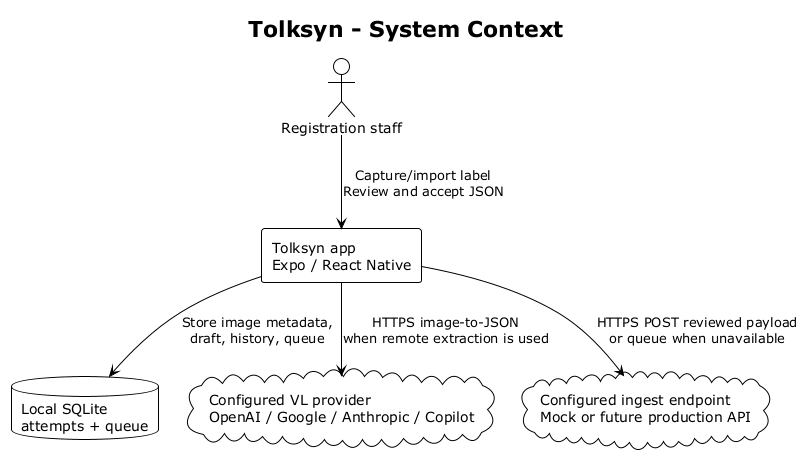
\includegraphics[width=0.92\textwidth,max height=0.58\textheight,keepaspectratio]{artifacts/system-context.png}
  \caption{System context diagram: registration staff capture a product label, review the extracted structured data, and send a JSON payload to an ingest endpoint while configured model providers handle image-to-JSON extraction.}
  \label{fig:system-context}
\end{figure}


% Background chapter in 'chap-background.tex'
\chapter{Background}
\label{chap:background}

\section{Mobile Application Platform}

The prototype is built as a React Native application. React Native enables native mobile interfaces using JavaScript and React concepts \cite{react-native}. Expo, an open-source framework built on top of React Native, was selected because the project needs camera access, image import, SQLite persistence, secure storage, and web support without introducing native modules or custom development clients. Expo Router provides file-based routing for React Native and web applications, which matches the required Capture, Confirm and Edit, History, and Settings screens \cite{expo-router}.

\section{Vision-Language Extraction}

The core recognition problem is not only optical character recognition. Product labels contain layout, abbreviations, model numbers, manufacturer names, country information, barcodes, and sometimes technical identifiers. A pure OCR pipeline can transcribe characters, but would still need a downstream mapping layer to decide which recognized text belongs to which registration field. The implementation therefore uses a vision-language extraction step to map visible label evidence directly into a structured JSON schema.

This distinction matters because transcription and registration are different tasks. OCR can make label text machine-readable, but inventory registration also requires field selection, normalization, and omission of values that are not visible or reliable. The project therefore treats model output as draft structured data, while deterministic barcode decoding, schema validation, and human review remain separate control points.

Planning still considered OCR and text-recognition approaches. CRNN represents neural scene-text recognition for image-based sequences \cite{crnn}, while Tesseract represents a classical OCR engine that was relevant as a baseline OCR option \cite{tesseract}. Gemini document processing and ML Kit Text Recognition v2 were also relevant practical options during planning \cite{gemini-doc-processing,mlkit-text-recognition}. These sources informed the design direction, but the implementation keeps deterministic barcode decoding separate and uses a VLM-first extraction boundary for schema mapping.

\section{Architecture Documentation}

The project uses C4-style architecture thinking, where the system is described through increasingly detailed views such as context, containers, components, and code \cite{c4-model}. The diagrams in this report are generated from PlantUML sources and rendered for inclusion in the report. Only the rendered diagram assets are included in the appendix and final report. The PlantUML source files remain project working files.

\section{Related Implementation Constraints}

The Expo managed workflow shaped the implementation. It supports portability across iOS, Android, and web, but it also discourages custom native model runtimes. For that reason, local vision-language inference remains future work. The current prototype prioritizes a reliable remote provider boundary, local persistence, human review, and replay-safe submission.

\chapter{Methodology}
\label{chap:methodology}

\section{Methodological Approach}

The project was carried out as an iterative software engineering project. The business problem was known from the start: Buy2Sell wanted to reduce manual registration work by scanning product labels and extracting useful registration data. The technical solution was uncertain. The team had to determine which fields could be extracted safely, how model output should be controlled, and how the application should behave when extraction or submission failed.

\begin{figure}[H]
  \centering
  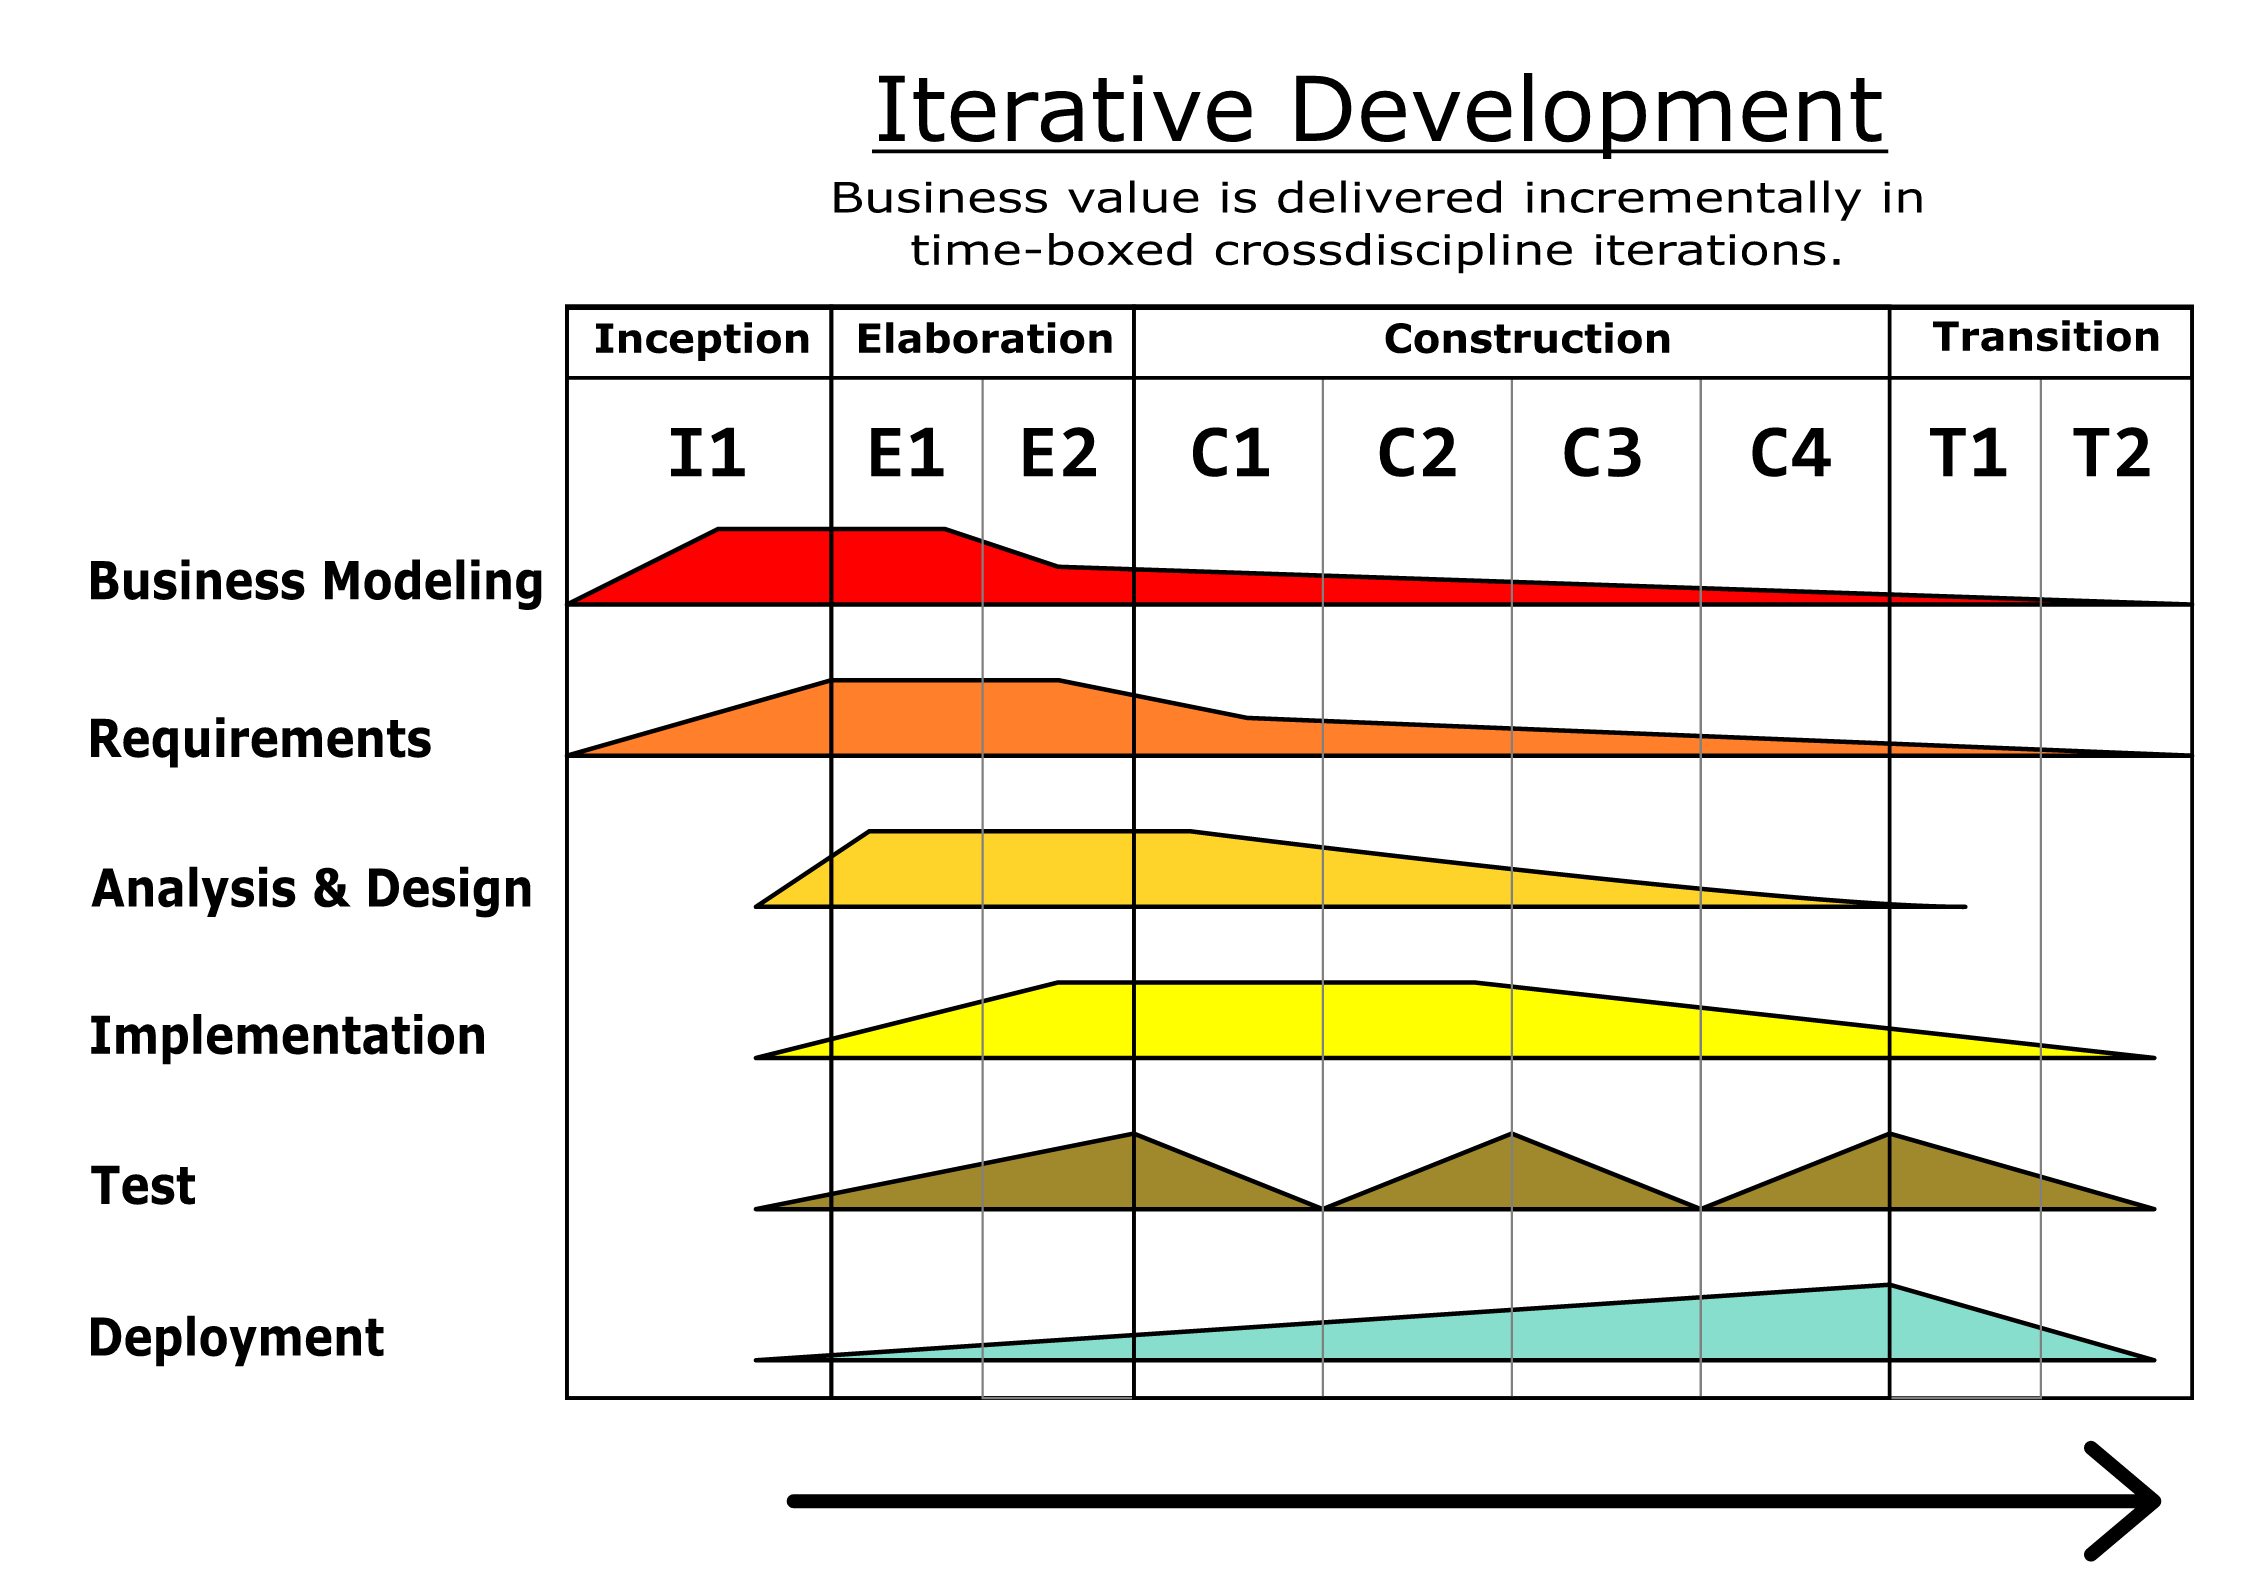
\includegraphics[width=0.9\textwidth,max height=0.58\textheight,keepaspectratio]{artifacts/unified-process-model.png}
  \caption{Unified Process-style lifecycle model showing time boxes and the change of focus over time.}
  \label{fig:unified-process}
\end{figure}

Figure~\ref{fig:unified-process} shows a Unified Process-style lifecycle model applied to the project's software development lifecycle. The model organized recurring disciplines such as requirements, design, implementation, validation, and documentation. The sprint workflow turned those disciplines into short implementation increments with concrete deliverables.

\begin{table}[H]
\centering
\begin{tabularx}{\textwidth}{P{0.20\textwidth}YY}
\toprule
\textbf{Method element} & \textbf{Use in the project} & \textbf{Reason} \\
\midrule
Unified Process-style lifecycle & Used as an overall SDLC planning model with overlapping disciplines. & Requirements, design, implementation, and validation had to evolve together. \\
Sprint workflow & Used to divide the work into short increments. & The prototype needed frequent integration and adjustment as technical risks became visible. \\
Risk-driven development & High-risk workflow boundaries were implemented early. & Capture, extraction, validation, review, and submission had to work together. \\
\bottomrule
\end{tabularx}
\caption{Methodological approach used in the project.}
\label{tab:method-approach}
\end{table}

Table~\ref{tab:method-approach} summarizes the methodological elements and why they were chosen. In this thesis, Unified Process-style (Table~\ref{tab:glossary}) means an iterative process where requirements, design, implementation, and testing overlap rather than run as one-way handovers.

\section{Project Phases}

The work was divided into five practical phases. The phases were not strict handover points. Later implementation work still affected requirements and design, but the phase structure made the work easier to plan, implement, and document. Table~\ref{tab:project-phases} lists the phase outputs.

\begin{table}[H]
\centering
\begin{tabularx}{\textwidth}{P{0.15\textwidth}YYY}
\toprule
\textbf{Phase} & \textbf{Main question} & \textbf{Work performed} & \textbf{Output} \\
\midrule
Discovery & What problem should the prototype solve? & Analysed the project brief, meeting notes, label fields, and workflow constraints. & Scope, field list, initial requirements. \\
Foundation & Can the app support the basic workflow? & Created Expo project structure, routing, local storage, and capture/import flow. & Running app skeleton with persisted attempts. \\
Extraction & Can label evidence become structured data? & Added barcode detection, provider-based vision-language extraction, prompt contract, parsing, and schema validation. & Draft AI-generated structured JSON from label images. \\
Review and ingest & Can the user safely accept and send data? & Added Confirm and Edit screen, accepted payloads, HTTP submission, idempotency, and offline queue. & Reviewed payload submission flow. \\
Hardening & Is the prototype reliable enough to demonstrate? & Added settings, diagnostics, retry behavior, automated tests, and documentation. & Testable prototype and thesis evidence. \\
\bottomrule
\end{tabularx}
\caption{Project phases and outputs.}
\label{tab:project-phases}
\end{table}

\section{Requirements Elicitation and Refinement}

Requirements were collected from the external project brief, the Buy2Sell meeting, and implementation findings. The requirements were then organized into functional requirements, non-functional requirements, and KPI targets, as shown in Table~\ref{tab:requirement-sources}.

\begin{table}[H]
\centering
\begin{tabularx}{\textwidth}{P{0.19\textwidth}YY}
\toprule
\textbf{Source} & \textbf{Input} & \textbf{Resulting requirements} \\
\midrule
Project brief & Manual registration, OCR and barcode idea, manufacturer and model extraction. & Capture, barcode decoding, structured extraction, registration payload. \\
Buy2Sell meeting & Multiple images, remote processing first, simulated server, previous-value suggestions, answerable fields only. & Multi-image requirement, configurable ingest endpoint, review step, field filtering. \\
Implementation findings & Provider output may be malformed, network delivery may fail, browser barcode support varies. & Schema validation, retry handling, offline queue, diagnostics, fallback behavior. \\
\bottomrule
\end{tabularx}
\caption{Requirement sources and their effect on the prototype.}
\label{tab:requirement-sources}
\end{table}

\section{Key Engineering Decisions}

Several decisions were made during development because of project constraints, technology constraints, and workflow risks.

\begin{table}[H]
\centering
\begin{tabularx}{\textwidth}{P{0.20\textwidth}P{0.23\textwidth}YP{0.18\textwidth}}
\toprule
\textbf{Decision} & \textbf{Alternatives considered} & \textbf{Reason} & \textbf{Consequence} \\
\midrule
Use Expo managed workflow & Bare React Native, custom native modules. & Faster cross-platform development and access to camera, image picker, SQLite, and secure storage. & Local VLM execution was excluded from the prototype. \\
Use VLM-first extraction & OCR-only pipeline, OCR plus rules, OCR plus LLM. & The system needed field mapping, not only text transcription. & Provider output had to be validated and reviewed. \\
Keep barcode decoding separate & Let the VLM read barcodes from the image. & Barcode values are deterministic evidence when decoded successfully. & Barcodes are merged conservatively into the result. \\
Require human confirmation & Fully automatic submission. & Some fields are ambiguous or require operator judgement. & Submission only happens after user acceptance. \\
Use local queueing & Cancel submission on network error. & Workshop network and endpoint availability may vary. & Accepted payloads can be replayed later. \\
\bottomrule
\end{tabularx}
\caption{Key engineering decisions and consequences.}
\label{tab:key-decisions}
\end{table}

In Table~\ref{tab:key-decisions}, deterministic merge means that extracted values are combined using fixed rules: barcode evidence is deduplicated, preserved in enrichment fields, and used to suggest \path{eanOrUpc} only for compatible barcode types. Ambiguous barcode candidates are recorded as conflicts instead of silently overwriting structured fields.

\section{Development Workflow}

The development workflow followed the primary application loop. Each increment extended or hardened the path from image capture to reviewed payload submission.

\begin{table}[H]
\centering
\begin{tabularx}{\textwidth}{P{0.19\textwidth}YY}
\toprule
\textbf{Increment} & \textbf{Goal} & \textbf{Validation} \\
\midrule
Capture/import & Create attempts from camera or gallery images. & Manual test and capture pipeline tests. \\
Extraction & Produce structured JSON from image evidence. & Provider parser tests, retry tests, schema validation tests. \\
Barcode enrichment & Detect and merge barcode evidence. & Barcode detector tests and merge tests. \\
Review & Let the user inspect and edit draft data. & Manual acceptance test and component tests. \\
Submission & Send accepted payloads to an endpoint. & Ingest transport and submission service tests. \\
Offline queue & Preserve accepted payloads when delivery fails. & Queue repository and queue worker tests. \\
Settings & Configure providers, endpoint, and credentials. & Settings repository and provider catalog tests. \\
\bottomrule
\end{tabularx}
\caption{Development increments and validation methods.}
\label{tab:development-increments}
\end{table}

\section{Technology Selection}
\label{sec:technology-selection}

Technology choices were made according to the prototype goals: cross-platform mobile support, camera access, local persistence, configurable remote extraction, and a reviewable JSON submission flow.

\begin{table}[H]
\centering
\begin{tabularx}{\textwidth}{P{0.20\textwidth}P{0.28\textwidth}Y}
\toprule
\textbf{Area} & \textbf{Selected technology} & \textbf{Reason} \\
\midrule
Mobile runtime & Expo and React Native & Cross-platform mobile implementation with web support and managed access to device features. \\
Routing & Expo Router & File-based navigation that matched the application screens. \\
Language & TypeScript & Static checking for structured data and service boundaries. \\
Persistence & Expo SQLite and Drizzle ORM & Local storage for attempts, settings, queue items, and typed database access through an ORM layer. \\
Validation & Zod & Runtime validation of model output and internal payloads. \\
AI integration & AI SDK provider adapters & Common abstraction for provider-based vision-language extraction. \\
Testing & Jest and React Native Testing Library & Automated validation of services, repositories, utilities, and selected UI behavior. \\
\bottomrule
\end{tabularx}
\caption{Technology choices and rationale.}
\label{tab:technology-selection}
\end{table}

Table~\ref{tab:technology-selection} also reflects a key tradeoff: Expo managed workflow supports portability and fast development, but it makes custom native model runtimes difficult. For that reason, local vision-language inference was treated as future work rather than part of the prototype.

Drizzle ORM (Table~\ref{tab:glossary}) was selected to keep SQLite access typed and centralized in repository code, instead of spreading handwritten SQL across screens and services.

\section{Validation Strategy}

Validation was divided into implementation validation, acceptance validation, and KPI evaluation.

\begin{table}[H]
\centering
\begin{tabularx}{\textwidth}{P{0.23\textwidth}YY}
\toprule
\textbf{Validation level} & \textbf{Purpose} & \textbf{Evidence} \\
\midrule
Implementation validation & Check technical behavior of services, repositories, schemas, retries, and queueing. & Automated Jest tests, type checking, linting. \\
Acceptance validation & Check that the operator can complete the capture-review-send workflow. & Manual end-to-end walkthroughs. \\
KPI evaluation & Measure extraction accuracy and define separate timing targets. & Extraction accuracy requires a fixed label dataset and reviewed ground truth. Time reduction requires a separate timed operator comparison. \\
\bottomrule
\end{tabularx}
\caption{Validation levels used in the project.}
\label{tab:validation-levels}
\end{table}

Automated tests validate the implemented workflow under expected and failure conditions. Extraction accuracy is handled separately in Chapter~\ref{chap:validation} because it requires real label images, reviewed ground truth, and semantic comparison. Registration time reduction is also separate because it depends on operator behavior, correction speed, and manual-entry baseline measurements.

\section{Method Limitations}

The methodology was suitable for building a working software prototype, but it does not by itself prove production effect. The project validates technical feasibility: image capture, barcode enrichment, provider-based extraction, schema validation, human review, submission, and offline queueing. Full business validation still requires timed manual baselines, production-build measurements, and evaluation inside the production registration workflow.


% Analysis and Design chapter in 'chap-analysis-and-design.tex'
\chapter{Problem Analysis}
\label{chap:analysis}

\section{Current Workflow}

The registration flow described in the external project brief depends on manual transfer from manufacturer labels into a registration system \cite{buy2sell-brief}. The same label may contain manufacturer name, product number, product text, version, EAN or UPC, country of origin, quantity, dimensions, weight, and technical identifiers. Manual entry is flexible but slow. It also creates inconsistent spelling, missed barcodes, and rework when the same manufacturer or product family appears repeatedly.

\section{Technical Challenges}

Product labels are not uniform. They vary by manufacturer, age, condition, placement, glare, font size, angle, and physical wear. Some labels include dense barcodes while others include only text. A robust system therefore cannot rely on a single recognition technique. The implementation combines local barcode detection with semantic vision-language extraction. Barcode detection is deterministic and provider-independent, while the vision-language provider interprets the broader label context and maps text into the JSON schema.

\section{Human-in-the-Loop Requirement}

The goal is not to remove the operator from the registration process. Some fields, such as condition or notes about scratches, require judgement. The Confirm and Edit step is therefore central to the design. AI output becomes a draft, not an unreviewed source of truth. This approach minimizes the risk of hallucinated or misread fields while still reducing repetitive typing.

\section{Approach Selection}

The original project idea mentions computer vision, OCR, barcode reading, and agentic AI \cite{buy2sell-brief}. The selected approach combines deterministic barcode decoding with VLM-first schema mapping and human confirmation. Barcode scanning is reliable when a barcode is visible, but it cannot fill manufacturer, product text, country, quantity, or other label fields. OCR can transcribe text, but it still needs a rule layer or language-model layer to map recognized text into the registration schema, normalize values, and leave unsupported fields empty.

The implementation therefore focuses on vision-language extraction rather than OCR-only processing. Modern multimodal models can interpret label images and produce structured outputs, while the AI SDK standardizes provider integration across supported model backends \cite{ai-sdk}. Web barcode support is available through the Barcode Detection API, although MDN marks it as limited and experimental, so the web implementation includes fallback package support \cite{barcode-detection-api}. The result is a hybrid workflow: deterministic barcode evidence is merged separately, probabilistic VLM output is validated against the schema, and the operator confirms the final payload before submission.

\section{Stakeholder Analysis}

\begin{table}[htbp]
\centering
\begin{tabularx}{\textwidth}{>{\raggedright\arraybackslash}p{0.24\textwidth}XX}
\toprule
Stakeholder & Need & System response \\
\midrule
Workshop registration staff & Fast capture and fewer repeated typing tasks & Camera-first workflow, draft extraction, editable confirmation. \\
Inventory administration & Consistent structured fields for downstream systems & Versioned JSON schema, validation, required field mapping. \\
IT / system owner & Configurable provider, endpoint, and credential handling & Settings screen, BYOK provider support, secure store abstraction. \\
Business management & Reduced handling time and better resale throughput & Automation of label transcription with human acceptance. \\
Future integration partner & Stable ingest contract and replay-safe delivery & Idempotency keys, queue persistence, schema metadata. \\
\bottomrule
\end{tabularx}
\caption{Stakeholder needs and system response.}
\label{tab:stakeholders}
\end{table}

\section{Field Complexity}

The field list from the meeting notes includes SKU, manufacturer, product number, product text, product version, EAN or UPC, country of origin, packaging, condition, working condition, quantity, dimensions, HS code, item group, sending type, selling type, and notes \cite{meeting-notes}. Some fields are directly visible on labels, some are inferred from product context, and some should remain user-entered. The extraction flow handles this by exposing only answerable fields to extraction and leaving review-time correction to the operator.


\chapter{Requirements}
\label{chap:requirements}

\section{Requirements Elicitation}

The requirements were elicited from three sources. First, the external project brief describes the business problem and the initial project request: scan product labels using a phone or camera, recognize text and barcodes, extract fields such as model, type, and manufacturer, and populate registration fields to reduce time and typing errors \cite{buy2sell-brief}. Second, the Buy2Sell meeting records how the team refined the scope around phone capture, multiple images for split labels, vision-language extraction, manufacturer lookup as a nice-to-have, previous-value suggestions, omission of label printing, and a simulated server POST \cite{meeting-notes}. Third, the requirements register formalizes those needs as the complete requirement set \cite{requirements-register}.

\section{External Project Requirements}

The original request from Buy2Sell is the external project baseline. The company explained that staff currently enter manufacturer, product type or model, item category, condition, and country of origin manually, even though many of those details already exist on product labels \cite{buy2sell-brief}. Their requested solution should scan a product label, recognize text and barcodes, extract relevant information such as model, type, and manufacturer, and populate the registration system without unnecessary manual input. These needs became the initial functional requirements for capture, barcode decoding, structured extraction, confirmation, and ingest.

\section{Meeting Requirements}

The in-person meeting narrowed and improved the requirement set. The company noted that competitors use multiple images on a turntable, so split-label support was recorded as a planned Should requirement rather than as the demonstrated core flow. The meeting also clarified that a phone is a sensible capture device, that remote processing should be implemented first, that local processing can be considered later, and that the team should simulate a server by posting to a mock endpoint because production server access is unavailable \cite{meeting-notes}. The meeting also introduced quality-of-life requirements such as dropdown suggestions for previously entered manufacturers and a rule that only fields answerable from the label should be exposed to the model.

\section{High-Level Requirements}

The table below is the high-level requirement table used in the main thesis. The complete requirements register is embedded in Appendix~\ref{app:evidence}.

\begin{table}[htbp]
\small
\centering
\begin{tabularx}{\textwidth}{P{0.09\textwidth}YP{0.10\textwidth}Y}
\toprule
ID & Requirement & Priority & Acceptance summary \\
\midrule
FR-001 & Capture a product-label image with the device camera. & Must & User can open capture view, take a photo, store the image, and start extraction. \\
FR-002 & Import an existing label image. & Must & User can select an image, copy it into app storage, create an attempt, and start extraction. \\
FR-003 & Attach multiple images to one item. & Should & Planned extension: user can attach two or more images and review one merged result. \\
FR-006 & Decode visible barcodes. & Must & Supported barcodes return value and symbology. Missing barcodes do not block extraction. \\
FR-008 & Extract structured data using a schema-driven vision-language provider. & Must & Provider output conforms to the internal extraction schema. \\
FR-009 & Prevent unsupported field inference. & Must & Manual-only or absent fields remain blank rather than hallucinated. \\
FR-012 & Require confirmation and editing before submission. & Must & User cannot submit without visiting confirmation. Edited values are final. \\
FR-014 & Allow manual entry and correction. & Must & User can override required registration fields and add human-only information. \\
\bottomrule
\end{tabularx}
\caption{High-level requirements based on project needs and meeting refinements, part 1.}
\label{tab:high-level-requirements}
\end{table}

\begin{table}[htbp]
\small
\centering
\begin{tabularx}{\textwidth}{P{0.09\textwidth}YP{0.10\textwidth}Y}
\toprule
ID & Requirement & Priority & Acceptance summary \\
\midrule
FR-021 & Configure ingestion settings. & Must & POST endpoint and authentication settings persist across restarts. \\
FR-022 & Submit confirmed payloads by HTTP POST. & Must & Two-hundred responses mark attempts sent. Failures are recorded and queued or left unsent. \\
FR-023 & Queue accepted payloads offline. & Must & Failed or offline submissions are persisted and replayable. \\
FR-025 & Show a recent history of attempts. & Must & History lists recent attempts with status, timestamps, images, payloads, and errors. \\
NFR-002 & Reach confirmation quickly enough for workshop use. & Must & Target is confirmation within 6 seconds for at least 90 percent of attempts under reference conditions. \\
KPI-001 & Measure extraction accuracy. & Must & Target is at least 85 percent correct pre-review extraction for mandatory fields on an agreed held-out set. \\
KPI-002 & Define registration time-reduction evaluation target. & Should & Target for a timed operator study is at least 50 percent median time reduction compared with manual entry on the same label set. \\
\bottomrule
\end{tabularx}
\caption{High-level requirements based on project needs and meeting refinements, part 2.}
\end{table}

\section{Requirement Register Format}

The full register preserves these columns: ID, requirement description, category, priority, acceptance criteria, complexity, scope decision, test or verification method, and planned delivery phase. These columns make the requirements traceable from the business request through design, implementation, and validation.

\section{Prioritization and Scope}

Must requirements form the minimum viable prototype: image capture and import, barcode decoding, vision-language extraction, schema validation, confirmation, manual correction, provider settings, BYOK, secure storage, ingestion, offline queue, history, retention, export, mock server, target field set, platform support, performance, reliability, and security. Should requirements improve usefulness and robustness, such as preprocessing, multi-image support, confidence display, autocomplete from history, provider fallback, retry, metadata traceability, ground-truth quality, and timed operator comparison. Could requirements are desirable extensions such as provider benchmarking, confidence-focused UI, image or keyword search, and local vision-language experiments. Local vision-language processing was considered during planning but is not part of the current implementation because available edge-device performance, app size, cold-start cost, and Expo managed-workflow constraints make it a poor fit for this prototype.

\section{Verification Strategy}

The register links each requirement to a verification method. Functional requirements are checked with manual acceptance tests and integration tests. Technical requirements are checked with schema, normalization, mapping, repository, and provider tests. KPI requirements require evaluation datasets, per-field accuracy measurement, and time studies. Security requirements require code and configuration review and platform inspection. Transitional requirements are verified by deliverable review, demo execution, and handover completeness.


\chapter{Design}
\label{chap:design}

\section{Architecture Model}

The design is compatible with the C4 model, which describes software architecture through hierarchical abstractions: software systems, containers, components, and code \cite{c4-model}. For this project, one software system contains a mobile and web application container, local persistence, and external model and ingest systems. Inside the app container, responsibilities are distributed across screens, providers, services, repositories, and API route handlers.

Figure~\ref{fig:component-diagram} shows this separation explicitly, including how user-facing screens delegate business behavior to services and repositories.

\begin{figure}[H]
  \centering
  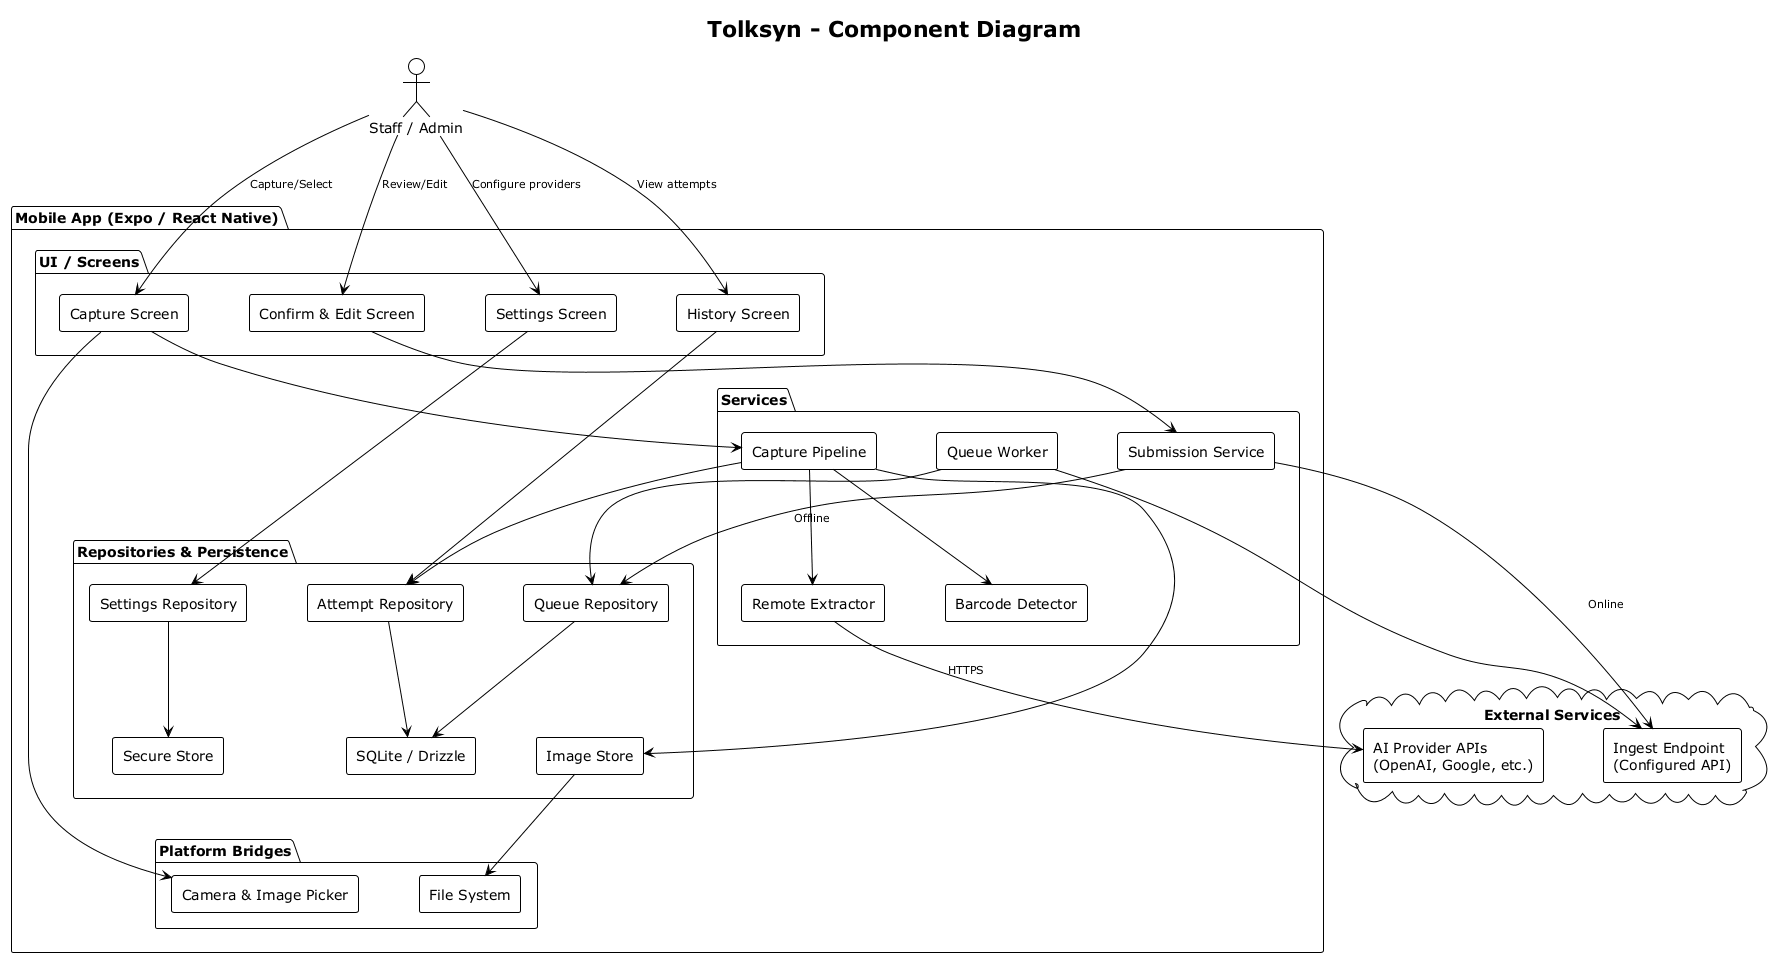
\includegraphics[width=0.95\textwidth,max height=0.58\textheight,keepaspectratio]{artifacts/component-diagram.png}
  \caption{Component diagram: routes and screens express user flow, while providers, services, repositories, and API modules handle runtime composition, persistence, extraction, and submission.}
  \label{fig:component-diagram}
\end{figure}

Table~\ref{tab:component-responsibility} complements this by listing the component boundaries and separation rationale.

\begin{table}[H]
\centering
\begin{tabularx}{\textwidth}{>{\raggedright\arraybackslash}p{0.25\textwidth}XX}
\toprule
Component & Responsibility & Reason for separation \\
\midrule
Screen modules & Render workflow state and collect user decisions & Keeps route files thin and UI focused. \\
App runtime provider & Composes database, settings, services, and queue worker & Central dependency wiring avoids scattered setup. \\
Capture pipeline & Coordinates image storage, barcode, extraction, merge, and persistence & Makes the end-to-end workflow testable. \\
Repositories & Read and write attempts, queue items, and settings & Isolates persistence details from business logic. \\
API routes & Proxy provider and web-search calls for web runtime & Keeps browser constraints away from screens. \\
\bottomrule
\end{tabularx}
\caption{Component responsibility model.}
\label{tab:component-responsibility}
\end{table}

\section{Capture-to-Ingest Pipeline}

The core pipeline distinguishes two evidence sources from the start: local barcode detection and provider-based vision-language extraction. Barcode detection is local and independent from provider routing, while the model provider only handles image-to-JSON extraction. The central design is deterministic: preprocess, run both extraction paths in parallel, merge, validate, confirm, then send.

Figure~\ref{fig:pipeline} visualizes this end-to-end loop.

\begin{figure}[H]
  \centering
  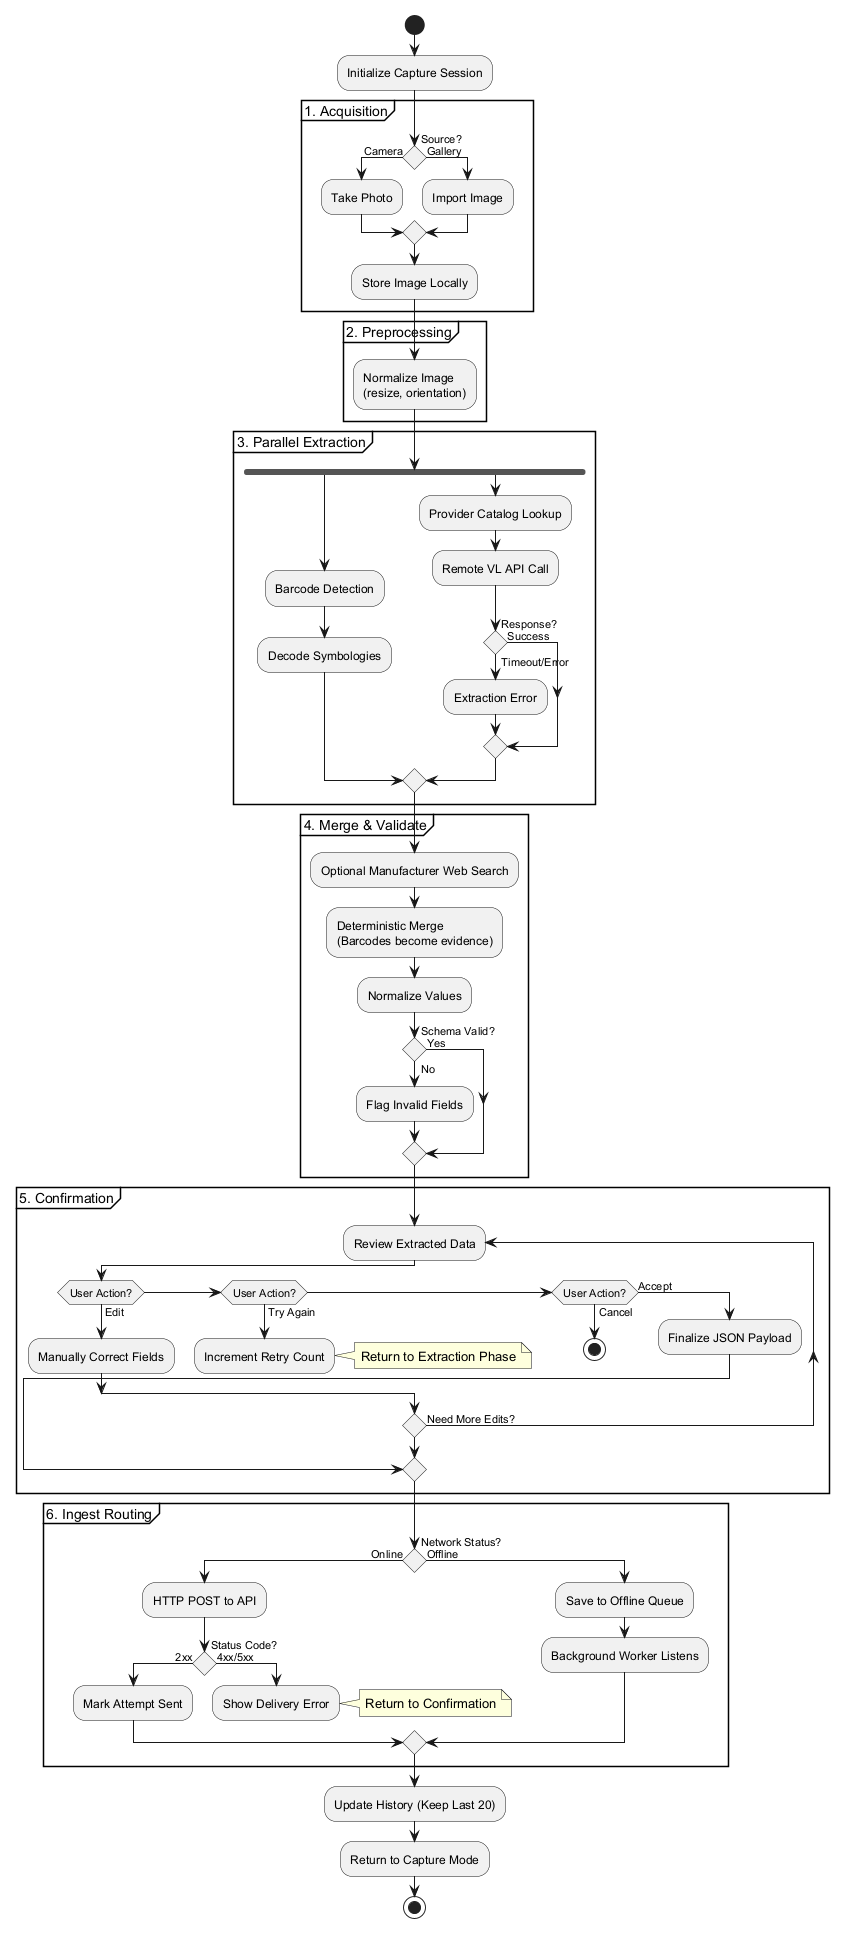
\includegraphics[height=0.78\textheight,max width=0.95\textwidth,keepaspectratio]{artifacts/app-pipeline-activity.png}
  \caption{Activity diagram: image storage, barcode detection, extraction, merge, validation, review, submission, and queueing are represented as one end-to-end capture-to-ingest workflow.}
  \label{fig:pipeline}
\end{figure}

The flow is:
\begin{itemize}
  \item user captures or imports an image,
  \item ImageStore normalizes the image and creates a thumbnail,
  \item AttemptRepository creates an attempt snapshot,
  \item barcode detection and remote extraction run in parallel,
  \item optional web-search enrichment adds manufacturer evidence,
  \item merge and validation produce a draft structured JSON object,
  \item the user edits and accepts the payload,
  \item SubmissionService sends immediately or queues with an idempotency key.
\end{itemize}

\section{Data Model}

Each capture is represented as an attempt. Attempt records store image URIs, timestamps, status, draft JSON, accepted revision, extraction result, and error code. Queue items store serialized payloads, retry state, idempotency keys, and attempt revision. Settings store non-secret configuration, while provider and ingest secrets are routed through the secret store abstraction. Figure~\ref{fig:persistence-model} shows the local data model used for this state.

\begin{figure}[H]
  \centering
  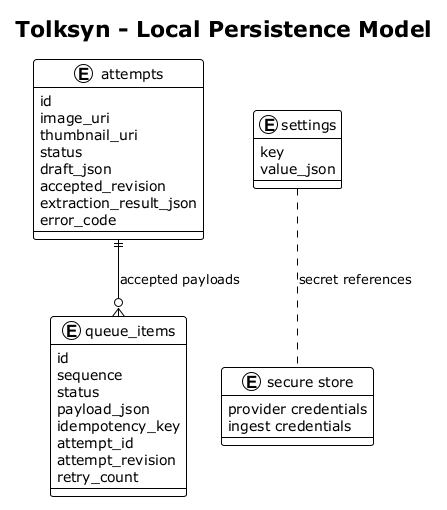
\includegraphics[width=0.88\textwidth,max height=0.62\textheight,keepaspectratio]{artifacts/local-persistence-model.png}
  \caption{Data model diagram: attempts, queue items, settings, and secure secret storage form the local state needed for review and replay.}
  \label{fig:persistence-model}
\end{figure}

\section{User Interface Design}

The user interface is organized around four main surfaces: Capture, Confirm and Edit, History, and Settings. Capture is optimized for fast repeated scans. Confirm and Edit gives the operator visibility into structured fields, barcode evidence, and diagnostics. History provides traceability for recent attempts. Settings makes the app portable across providers and ingest environments.

Figure~\ref{fig:ui-flow} summarizes the runtime navigation, while the design-stage Figma artifact is included as appendix evidence in Table~\ref{tab:evidence-artifacts}.

\begin{figure}[H]
  \centering
  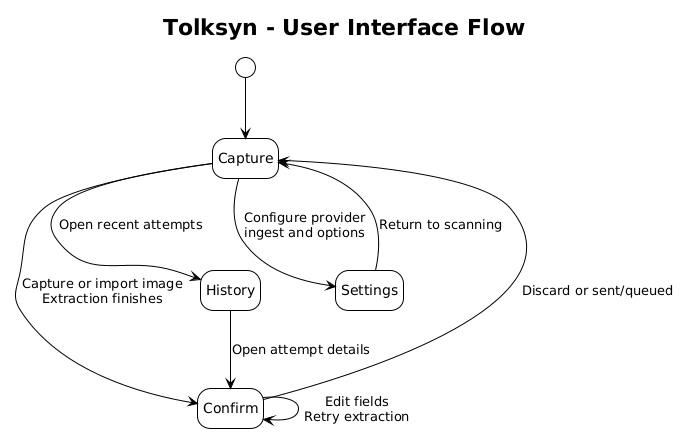
\includegraphics[width=0.92\textwidth,max height=0.58\textheight,keepaspectratio]{artifacts/ui-flow.png}
  \caption{User-flow diagram: navigation across Capture, Confirm and Edit, History, and Settings.}
  \label{fig:ui-flow}
\end{figure}

\section{Security and Privacy Design}

The project requires secrets to be stored securely, HTTPS for remote calls, no telemetry by default, and diagnostics with secret redaction. Expo SecureStore encrypts and securely stores key-value pairs locally on Android and iOS, using Android Keystore-backed encrypted SharedPreferences and iOS Keychain services \cite{expo-securestore}. The production deployment should enforce HTTPS ingest endpoints and ensure that web deployments apply the same secret-handling policy appropriate to the browser environment.

\section{State Model}

Attempt state is explicit. A typical attempt moves from \emph{captured} to \emph{ready for review}, then to \emph{sent} or \emph{queued} after user acceptance. Failure states distinguish \emph{extraction failed} from \emph{send failed}. Attempts that are sent, queued, or failed remain visible until retention pruning, while user-discarded and aborted partial attempts are removed from local history. This state model supports retry, history display, and queue replay without relying on transient UI state.

Figure~\ref{fig:state-model} shows the explicit transitions that support retry and queue replay behavior.

\begin{figure}[H]
  \centering
  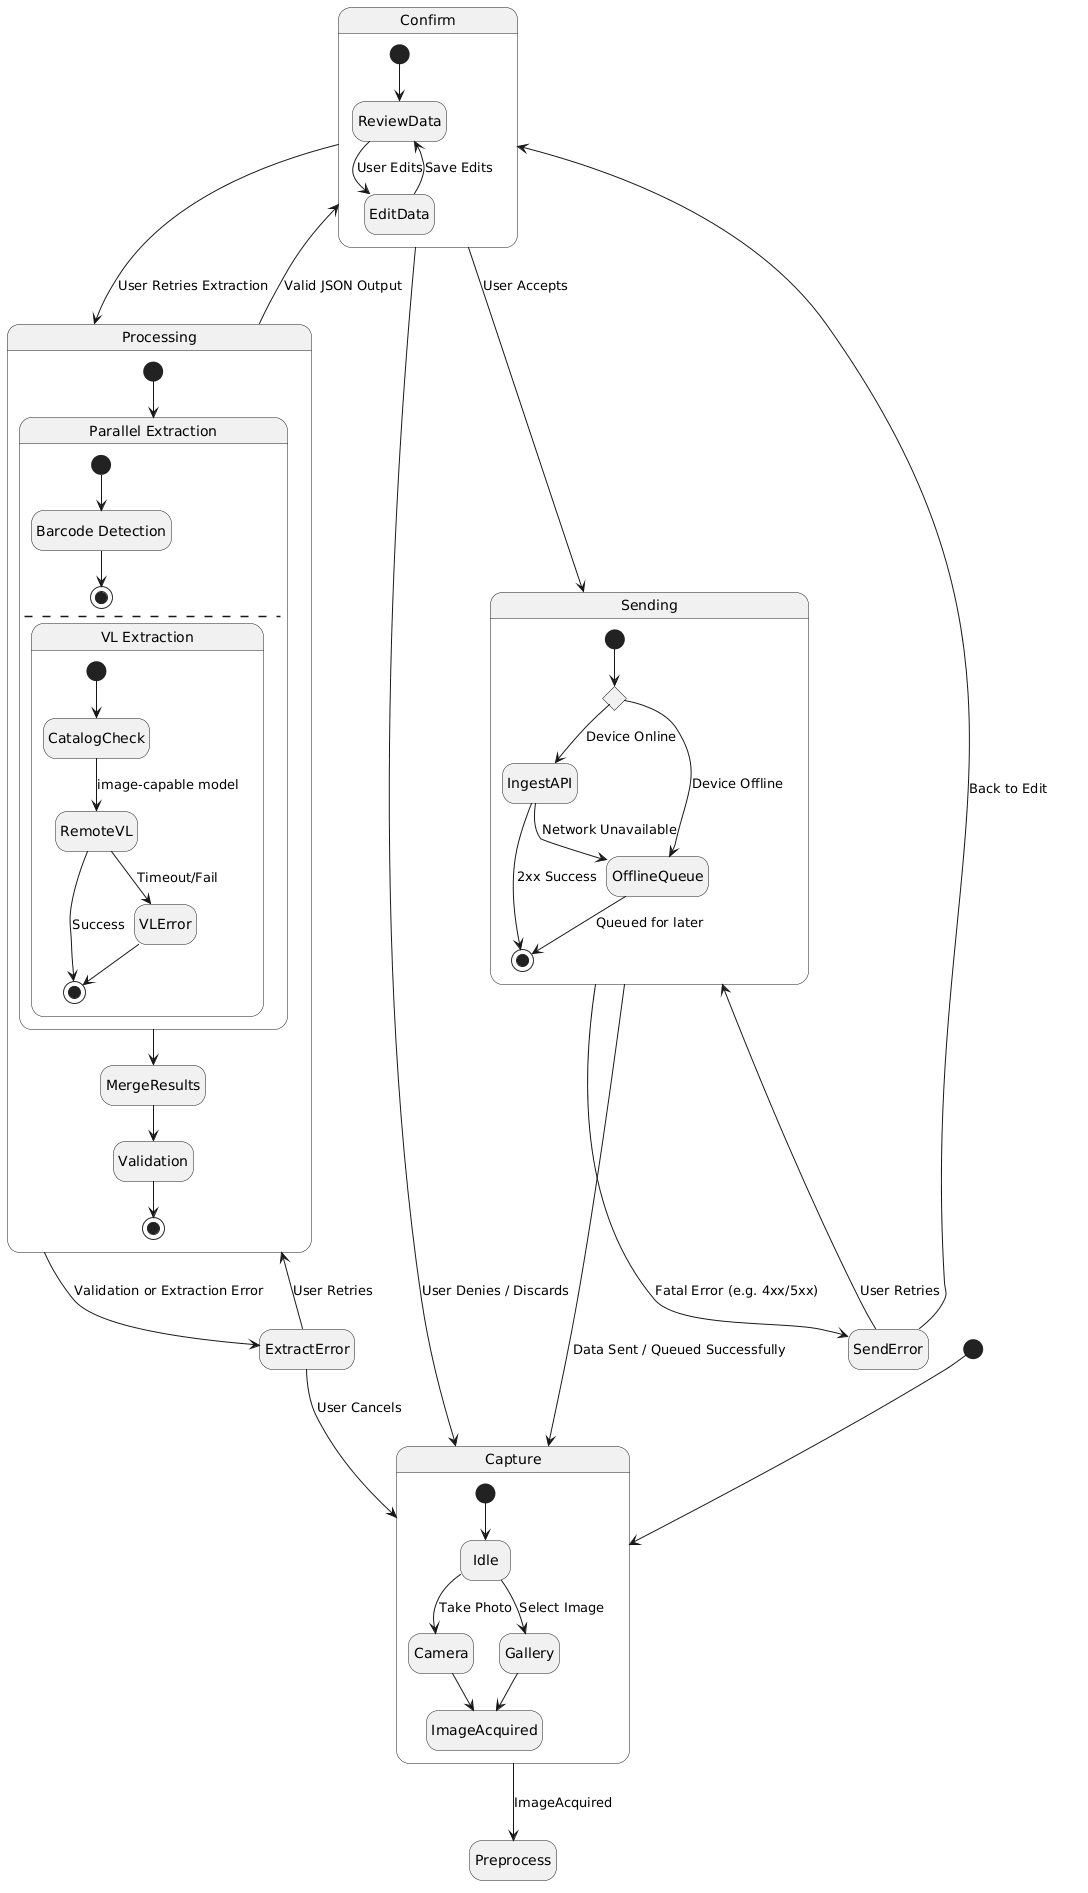
\includegraphics[height=0.78\textheight,max width=0.95\textwidth,keepaspectratio]{artifacts/app-state-machine.png}
  \caption{State-machine diagram: explicit attempt statuses make retry, history, discard, queueing, and delivery behavior visible.}
  \label{fig:state-model}
\end{figure}


% Implementation chapter in 'chap-implementation.tex'
\chapter{Implementation}
\label{chap:implementation}

\section{Application Runtime}

The runtime design solves a coordination problem: screens need camera, storage, extraction, queue, settings, and submission behavior, but the screens should not construct those dependencies themselves. The application therefore uses Expo Router for navigation and \path{AppRuntimeProvider} in \path{src/providers/app-provider.tsx} as the composition root \cite{expo-router}.

The provider creates the Drizzle database from the Expo SQLite context, constructs repositories, creates the provider catalog, image store, barcode detector, remote extractor, web-search enricher, ingest transport, submission service, and queue worker, then exposes the resulting runtime to screens \cite{drizzle,expo-sqlite}. Expo Camera supplies camera preview, photo capture, and barcode scanner support, while Expo ImagePicker provides the system UI for selecting existing images or taking a photo \cite{expo-camera,expo-imagepicker}.

The practical effect is that \path{src/screens/capture.tsx} can call \path{runtime.processImage} without knowing whether barcode detection is native or web-specific, whether settings are stored in SQLite or secure storage, or how the queue worker is wired. The tradeoff is that runtime creation becomes a central integration point. If a dependency is wired incorrectly, several flows can fail together. This risk is why repository, service, and API-route tests are more valuable here than isolated screen tests.

\section{Capture Pipeline}

As described in Chapter~\ref{chap:design}, the implementation keeps local barcode detection separate from provider-based vision-language extraction. The capture pipeline converts a captured label image into a stored extraction attempt. In \path{src/services/capture-pipeline.ts}, \path{processImage} performs this conversion in a fixed order:
\begin{itemize}
  \item create an attempt id,
  \item persist the normalized image,
  \item create an attempt record,
  \item run barcode detection and remote extraction concurrently,
  \item optionally run manufacturer web-search enrichment,
  \item merge the evidence,
  \item save the resulting extraction record.
\end{itemize}

The concurrency is deliberate. Barcode decoding and VLM extraction use the same persisted image but do not depend on each other, so \path{processImage} starts both with \path{Promise.all}. This reduces the time needed to reach the confirmation screen from \path{barcode_time + extraction_time} to \path{max(barcode_time, extraction_time)}, assuming the device and network can execute barcode detection and label extraction concurrently. The code also treats the two tasks differently when they fail. Barcode failure is logged and returns an empty list because missing barcode evidence should not block human review. Extraction failure becomes a fallback structured item with diagnostics because the confirmation screen still needs an attempt to display and a failure reason to explain.

Abort handling is another important implementation detail. \path{processImage} checks the abort signal after persistence, attempt creation, barcode and extraction completion, enrichment, and before saving. If the user cancels after an attempt has been created, the catch block deletes the partial attempt through \path{attempts.deleteById}. This prevents abandoned records from polluting history while still allowing failed extraction attempts to remain visible when they are useful for diagnosis.

\section{Barcode Detection}

Barcode decoding is separated from VLM extraction because the two techniques have different reliability profiles. A barcode is a machine-readable symbol with a deterministic payload, whereas a VLM is a probabilistic text generator that may infer or format values incorrectly. The application therefore treats decoded barcodes as independent evidence rather than as text that the model must rediscover.

On native platforms, \path{src/services/barcode-detector.ts} uses Expo Camera's \path{Camera.scanFromURLAsync} to scan the persisted image \cite{expo-camera}. On web, \path{src/services/barcode-detector.web.ts} first tries the browser Barcode Detection API and falls back to the \path{barcode-detector} package when the native browser API is unavailable. The web implementation also limits image fetches with content-type, size, and timeout checks. MDN marks the Barcode Detection API as limited and experimental, so the fallback is needed for portability across browsers \cite{barcode-detection-api}.

The merge rule in \path{src/utils/merge-extraction-result.ts} is conservative and deterministic. \path{mergeExtractionResult} deduplicates barcodes by type and data, stores the first decoded value as primary evidence, and suggests \path{eanOrUpc} only for barcode types that are semantically appropriate for retail identifiers. It does not automatically overwrite unrelated structured fields with barcode text. If multiple EAN/UPC candidates exist, it records a conflict instead of silently choosing one. This is a direct human-in-the-loop tradeoff: preserve evidence and let the user resolve ambiguity instead of hiding uncertainty in an automatic field overwrite.

\section{Vision-Language Extraction}

The extraction boundary implements the distinction described in Chapter~\ref{chap:background}: the app needs structured registration fields, not only transcribed text. The implementation therefore uses a remote, schema-constrained vision-language extraction step rather than a local OCR pipeline \cite{ai-sdk}.

The prompt contract is defined in \path{src/api/providers/extraction-prompt.ts}. It requires one complete JSON object, with top-level keys \path{structured_json} and \path{auxiliary_text_optional}, and requires every schema field to appear exactly once. Unknown values must be null. This null policy is important: it converts missing evidence into explicit absence, which can be validated and reviewed, instead of encouraging the model to infer manual-only fields such as condition.

The code does not rely on the model to be correct. \path{src/api/remote-extractor.ts} reads the selected provider and auth mode from settings, verifies image support through the provider catalog, and then calls the Vercel AI SDK \path{generateText} function with a single user message containing a text prompt and a file part containing the image base64 and media type. Provider retries are set to zero there so provider-level retry behavior does not hide malformed outputs from the application-level repair loop \cite{ai-sdk}.

The response is parsed by \path{parseProviderJsonEnvelope} in \path{src/api/providers/remote-extraction-shared.ts}. The parser rejects empty text, malformed JSON, a missing \path{structured_json} object, and schema-invalid structured data. It then normalizes the optional auxiliary text. This makes the VLM boundary explicit: provider text is untrusted until JSON parsing and Zod validation succeed \cite{zod}. The limitation is that the app validates shape and types, not semantic truth. A schema-valid but wrong manufacturer name still requires user review or dataset-based accuracy evaluation.

\section{Provider Catalog and Settings}

Provider model metadata changes over time. Image-capable model lists change faster than the application should be released, but the app still needs safe defaults when metadata services are unavailable. The function \path{createProviderCatalog} in \path{src/services/provider-catalog.ts} fetches provider metadata, normalizes providers, filters deprecated models, checks image support, caches results for five minutes, and falls back to built-in defaults for OpenAI, Google, Anthropic, and GitHub Copilot.

The catalog is not a generic model marketplace. \path{SUPPORTED_EXTRACTION_PROVIDER_IDS} restricts extraction to the providers for which the project has adapter code in \path{src/api/remote-extractor.ts}. A model may appear in a metadata service but still be unusable if the application does not know how to authenticate and call that provider through the AI SDK. The consequence is controlled configurability: users can change providers and models, but only inside the boundary the implementation can actually execute.

Settings also carry a security tradeoff. Provider credentials and ingest keys are required for BYOK operation (Table~\ref{tab:glossary}), but they must not be mixed with ordinary JSON settings. \path{src/repositories/settings-repository.ts} stores non-secret configuration separately from provider auth and ingest API material. This aligns with the SecureStore design in the architecture \cite{expo-securestore}, while still acknowledging a platform limitation: web environments cannot provide the same native Keychain/Keystore guarantees as iOS and Android.

\section{Manufacturer Web Search}

Manufacturer web-search enrichment is optional because external web evidence can conflict with label-derived evidence. The feature is implemented in \path{src/services/manufacturer-websearch.ts} with the project dependency \path{agent-query-crawl}. The runtime composition in \path{src/providers/app-provider.tsx} dynamically loads \path{createAgentQueryCrawl} only when the feature is used and configures web proxy routes for Exa search and page fetching through \path{src/app/api/proxy/exa/mcp+api.ts} and \path{src/app/api/proxy/webfetch+api.ts}.

The enrichment flow has two model-controlled steps around one deterministic crawl step. First, the extractor plans at most three search queries from the current structured JSON, barcode evidence, auxiliary text, and raw model response. Second, \path{agent-query-crawl} executes those queries and fetches at most six source pages in total. Third, the extractor reconciles the fetched evidence with the original extraction. The service sanitizes untrusted web text before reconciliation and records diagnostics for query planning, search, page fetches, field changes, and conflicts.

The reconciliation prompt gives priority to the original label/image extraction and decoded barcodes. Web evidence may fill null or ambiguous fields, or corroborate a correction, but it should not override label evidence without a conflict note. This keeps the web-search package as an enrichment aid rather than a second source of truth. The tests in \path{tests/services/manufacturer-websearch.test.ts} cover query planning, passing queries to \path{agent-query-crawl}, reconciliation, skipped searches when no queries are returned, and the shared crawl-page limit.

\section{Persistence}

Persistence is used for two different reasons: traceability and recovery. An attempt records what happened during a capture, while a queue item records work that still has to be delivered. \path{src/db/schema.ts} defines attempts, queue items, and settings. \path{src/repositories/attempt-repository.ts}, \path{src/repositories/queue-repository.ts}, and \path{src/repositories/settings-repository.ts} hide the SQL details from services.

The Drizzle and SQLite combination gives the application a typed database boundary while keeping the data local to the app \cite{drizzle,expo-sqlite}. This matters because the same repository methods can be tested without screens knowing about SQL statements, and because queue replay depends on stable ordering rather than transient React state.

The attempt repository also implements retention. The project requirement keeps only the latest 20 attempts, and \path{RuntimeLimits.historyLimit} encodes that value. The reason is operational rather than theoretical: label images are large compared with structured JSON, so unlimited history would eventually conflict with the data minimization requirement. The limitation is that retention reduces local audit history. A production deployment would need a backend audit store if long-term traceability is required.

\section{Schema Validation}

Validation is the boundary between model output and deterministic application state. \path{src/types/item-schema.ts} defines text fields such as manufacturer, product number, EAN or UPC, and country of origin, and numeric fields such as quantity, price, and dimensions. \path{normalizeStructuredItemInput} converts empty text to null, parses numeric-like strings to numbers when possible, and preserves invalid numeric text so validation can reject it. \path{validateStructuredItem} then reports numeric field errors and validates links before running the final Zod object schema \cite{zod}.

This design is stricter than simply accepting any provider JSON but more flexible than requiring every field to be present in the provider response. \path{parseProviderJsonEnvelope} merges provider output with \path{emptyStructuredItem}, so missing schema fields become explicit nulls before validation. The consequence is that the confirmation screen can always reason over the same object shape. The tradeoff is that schema validation cannot prove that a value was visible on the label. It only proves that the value has an acceptable type and field name. Semantic correctness still depends on human review and future evaluation datasets.

The retry mechanism in \path{src/services/extraction-retry.ts} is built around this validation boundary. It attempts extraction up to the configured maximum, currently three. Retryable failures are limited to schema violations, invalid responses, internal errors, and extraction-fallback errors. On the next attempt, the repair prompt adds the previous error and repeats the instruction to return one valid JSON object with no markdown or prose. After the last retry, the service returns an empty structured item with diagnostics. This preserves the user journey while making the failure visible instead of silently hiding it.

\section{Submission and Offline Queue}

Submission begins only after human acceptance because the accepted payload becomes the version that can leave the device. \path{src/services/submission-service.ts} builds around a submission payload containing the schema version, attempt id, accepted revision, structured JSON, barcode enrichment, optional auxiliary text, and metadata. The stable idempotency key is generated from attempt id and accepted revision through \path{src/utils/idempotency.ts}. This means the same accepted revision produces the same key across retries, while a later edited revision can produce a different key.

The ingest transport in \path{src/api/ingest-transport.ts} classifies delivery outcomes before the queue sees them. Missing endpoint configuration and missing API keys are permanent errors because retrying will not fix them. HTTP 408, 429, and 5xx responses are retryable because they represent timeout, rate limiting, or server/network instability. Other 4xx-style failures become permanent invalid responses or auth failures. This classification matters because retrying permanent errors would consume battery and network while keeping a bad item at the head of the queue.

Queue replay is intentionally FIFO. \path{drainQueue} in \path{src/services/queue-worker.ts} repeatedly calls \path{peekReady}, submits the head item, marks successes sent, marks permanent failures failed, and reschedules a retryable item with a later next attempt time. On a retryable failure it stops instead of skipping to later items. This preserves submission order, which is useful if the backend eventually treats attempts as a chronological registration stream.

\section{Implementation File Map}

\begin{table}[H]
\centering
\begin{tabularx}{\textwidth}{>{\raggedright\arraybackslash}p{0.20\textwidth}XX}
\toprule
Area & Important files & Purpose \\
\midrule
Routes & \path{src/app/_layout.tsx}, \path{src/app/(tabs)}, \path{src/app/confirm/[attemptId].tsx} & Navigation, root providers, route-to-screen mapping. \\
Screens & \path{src/screens/capture.tsx}, \path{confirm.tsx}, \path{history.tsx}, \path{settings.tsx} & User workflows and screen state. \\
Extraction & \path{src/api/remote-extractor.ts}, \path{src/api/providers/*} & Prompt construction, provider calls, response parsing. \\
Services & \path{src/services/capture-pipeline.ts}, \path{submission-service.ts}, \path{queue-worker.ts} & Business process orchestration. \\
Persistence & \path{src/db/schema.ts}, \path{src/repositories/*}, \path{drizzle/*} & SQLite schema, migrations, repository interfaces. \\
Types & \path{src/types/item-schema.ts}, \path{app-error.ts}, \path{settings.ts} & Shared contracts, validation, settings defaults. \\
Tests & \path{tests/services}, \path{tests/repositories}, \path{tests/types}, \path{tests/components} & Risk-based automated checks. \\
\bottomrule
\end{tabularx}
\caption{Implementation file map.}
\label{tab:implementation-map}
\end{table}


\chapter{Validation}
\label{chap:validation}

\section{Testing Strategy}

Testing follows the project preference for high-value integration and contract tests. Jest is the configured test runner, and Jest's standard workflow supports running tests through a package script \cite{jest}. React Native Testing Library supports tests that resemble user interaction rather than implementation details \cite{rntl}. The project also uses \path{jest-expo} so Expo and React Native modules can be tested in the app context.

Integration tests are preferred over narrow unit tests for most behavior because the highest risks sit between modules: camera or gallery input becomes persisted image data, extraction and barcode results are merged, queue items survive repository boundaries, and settings change provider behavior. Isolated unit tests are still useful for pure schema, merge, retry, and idempotency functions, but many Expo APIs require mocks under \path{jest-expo}. Testing only mocked internals would give weak evidence, so the suite emphasizes service, repository, API-route, and UI component boundaries.

\section{Automated Coverage Areas}

The repository contains tests for provider catalog behavior, extraction retry, OAuth flows, manufacturer web search, settings repositories, secure store behavior, queue worker logic, queue replay, capture pipeline, gallery import, barcode detection, submission, toast state, schemas, idempotency, retry policy, and selected UI components. This coverage aligns with the risks in the primary loop: model failure, offline behavior, malformed JSON, queue consistency, and user confirmation, which Table~\ref{tab:validation-matrix} maps to representative tests.

\begin{table}[htbp]
\centering
\begin{tabularx}{\textwidth}{>{\raggedright\arraybackslash}p{0.22\textwidth}>{\raggedright\arraybackslash}p{0.34\textwidth}X}
\toprule
Area & Representative tests & Validated behavior \\
\midrule
Capture pipeline & \path{capture-pipeline.test.ts}, \path{gallery-import.test.ts} & Image processing, attempt creation, extraction, barcode merge, retry handling. \\
Provider integration & \path{provider-catalog.test.ts}, \path{extraction-retry.test.ts}, \path{provider-oauth.test.ts} & Model discovery, fallback behavior, auth device flows, invalid responses. \\
Queue and ingest & \path{queue-worker.test.ts}, \path{queue-replay.integration.test.ts}, \path{submission-service.test.ts} & Offline queueing, FIFO drain, retry scheduling, idempotent submission. \\
Persistence & \path{attempt-repository.test.ts}, \path{queue-repository.test.ts}, \path{settings-repository.test.ts} & Repository CRUD behavior, settings persistence, status transitions. \\
Schema and utilities & \path{item-schema.test.ts}, \path{idempotency.test.ts}, \path{retry-policy.test.ts} & Runtime validation, stable keys, backoff and merge behavior. \\
UI components & \path{button.test.tsx}, \path{diagnostic-disclosure.test.tsx} & Reusable component rendering and user-facing diagnostic display. \\
\bottomrule
\end{tabularx}
\caption{Validation matrix.}
\label{tab:validation-matrix}
\end{table}

The tests are most useful where they verify behavior across a boundary. \path{tests/services/capture-pipeline.test.ts} exercises the same orchestration used by the Capture screen. The test suite checks that attempts are created after image persistence, that extraction and barcode evidence are merged, that web-search enrichment can update diagnostics, that enrichment failure does not destroy the original extraction, and that aborting after attempt creation removes the partial attempt. This directly validates the pipeline consequence described in Chapter~\ref{chap:implementation}: the user should either receive a reviewable attempt or a controlled cancellation, not a hidden half-written record.

The extraction tests validate the model-output boundary. \path{tests/api/remote-extractor.test.ts} checks that the AI SDK call contains both the text prompt and image file part, and that missing credentials or unsupported image models fail before a provider call is attempted. \path{tests/services/extraction-retry.test.ts} verifies the repair-loop behavior: invalid or schema-breaking model output records diagnostics and is retried, while final exhaustion returns an empty fallback structured item rather than throwing an unhandled error through the UI. These tests do not prove extraction accuracy. They prove that malformed provider behavior is contained.

The persistence and queue tests validate recovery assumptions. \path{tests/repositories/queue-repository.test.ts} and \path{tests/services/queue-worker.test.ts} check the queue head, retry scheduling, sent/failed transitions, and ordering. \path{tests/services/queue-replay.integration.test.ts} covers the combined replay path. \path{tests/api/ingest-transport.test.ts} checks HTTP outcome classification, including retryable statuses and permanent auth/configuration failures. Together these tests support the claim that accepted payloads are not discarded when delivery is temporarily unavailable. They do not prove behavior against a real production backend. That remains outside the prototype boundary.

\section{Acceptance Validation}

Acceptance validation focuses on the full operator journey: open Capture, grant camera permission, capture or import a label, wait for extraction, review fields, correct uncertain values, accept, and verify that the attempt is sent or queued. The most important acceptance criterion is that the user can finish registration without manually retyping every visible label field.

\section{Performance and Reliability}

The requirements target confirmation within 6 seconds for most attempts under stable network conditions, UI response under 100 ms, and cold start under 3 seconds \cite{requirements-register}. The architecture supports these targets by parallelizing barcode detection and model extraction, keeping local persistence lightweight, limiting history to 20 attempts, and using background queue replay rather than blocking the review flow on network availability.

\path{processImage} reduces one avoidable delay by running barcode detection and extraction in parallel, and the image store reduces image size by normalizing to a 1200 px wide WebP plus a thumbnail. The dominant latency still depends on remote provider response time, network conditions, image content, and selected model. The empirical KPI evaluation in Section~\ref{sec:kpi-evaluation} therefore focuses on extraction correctness, while automated tests validate the reliability behavior around retries, fallback responses, and queue preservation.

Lighthouse reports for the Capture, Confirm, History, and Settings routes are retained in Appendix~\ref{app:lighthouse}. Low web performance scores from these captures should be interpreted cautiously because the Expo development server does not apply the same compression, minification, tree-shaking, and static asset handling as a production web export. The Lighthouse artifacts are useful for accessibility, best-practice, and route inspection evidence, while the KPI evaluation provides separate evidence for extraction correctness.

\section{KPI Evaluation}
\label{sec:kpi-evaluation}

An empirical evaluation was performed to test KPI-001, the pre-review extraction-accuracy requirement, against Buy2Sell product-label images. The evaluation used 88 NDA-protected images originating from Buy2Sell. The original images are not embedded in the thesis because they may contain company-sensitive information. Instead, Appendix~\ref{app:kpi-evidence} contains anonymized per-image and per-field result evidence.

The measured quantity is field-level semantic correctness. This is the appropriate unit because different labels expose different facts: a label may show a manufacturer and product number but no country of origin, while another may include quantity, item group, or a reference code. Counting every schema field for every image would incorrectly penalize the extractor for fields that are not visible. The denominator is therefore the number of visible, answerable fields that entered the review set. Manual-only registration fields, such as condition and working condition, were excluded because they are not label-evidence fields.

The evaluation follows the same extraction contract implemented in the application. The prompt contract in \path{src/api/providers/extraction-prompt.ts} requires one parseable JSON object with \path{structured_json} and \path{auxiliary_text_optional}. The parser in \path{parseProviderJsonEnvelope} accepts provider output only after JSON parsing and schema validation. The schema normalization in \path{src/types/item-schema.ts} converts empty text to \path{null}, normalizes numeric fields, and keeps the same structured shape for every attempt. This matters for the KPI: schema validation can prove that an output has the right keys and types, but it cannot prove that a manufacturer, product number, or reference value is true. The KPI evaluation supplies that semantic check by comparing the normalized extraction output against reviewed label evidence.

The OpenAI provider was configured with \path{gpt-5.3-codex}. This is a powerful vision-language model, and that model choice likely improves the extraction result compared with weaker or cheaper models. The measured result should therefore be read as the outcome for this provider and model configuration. The system appears especially accurate when the image is sharp and the product label is visible in the frame, because the model receives both the text prompt and the image evidence needed to map visible label content into the JSON schema. Most observed failures were linked to blurred or unclear images.

The scoring process used normalized field comparison followed by semantic adjudication for non-exact matches. Exact string or numeric matches were counted directly. Barcode-like and code-like fields were normalized so that harmless punctuation or spacing differences did not create false errors. Where a value differed textually but appeared semantically equivalent, the discrepancy was recorded and adjudicated as correct or incorrect. Examples include formatting differences in version codes or non-material prefix and suffix differences in product numbers. This prevents the metric from treating every character-level difference as a product-registration error while still preserving a field-level discrepancy record in the anonymized evidence.

The review phase produced correction files for 18 images. In this evaluation context, a correction means that at least one VLM-extracted field for that image was changed to match information visible in the image. It does not mean that the reviewer added new registration information outside the label evidence. The activity is therefore comparable to the application's confirmation screen because both involve checking extracted fields, but the KPI measurement is narrower: it scores only whether the VLM extraction matched the visible label. If no correction was present, the extraction was treated as accepted after review. Manual review is itself a measurement step: reviewing 88 images and their corresponding JSON outputs is detailed work, and reviewer fatigue or human oversight can affect whether every small mistake is noticed. Some incorrect or partially incorrect fields may therefore have been missed. The statistic should therefore be interpreted as the measured result of this reviewed evaluation procedure, with human review forming part of the measurement method, as summarized in Table~\ref{tab:kpi-evaluation-setup}.

\begin{table}[htbp]
\centering
\begin{tabularx}{\textwidth}{P{0.32\textwidth}Y}
\toprule
\textbf{Evaluation setting} & \textbf{Value} \\
\midrule
Evaluation images & 88 Buy2Sell product-label images \\
Provider & OpenAI \\
Model & \path{gpt-5.3-codex} \\
Extraction mode & Remote vision-language extraction \\
Barcode handling & Local barcode detection merged before review \\
Scoring method & Normalized field-level comparison with semantic adjudication for non-exact matches \\
Evidence artifact & Anonymized KPI result PDF in Appendix~\ref{app:kpi-evidence} \\
\bottomrule
\end{tabularx}
\caption{KPI evaluation setup.}
\label{tab:kpi-evaluation-setup}
\end{table}

The evaluation measured pre-review extraction accuracy for KPI-001, shown in Table~\ref{tab:kpi-extraction-accuracy}. Accuracy was computed as the number of correct scored fields divided by the total number of scored fields. A field entered the denominator only when it was present in the reviewed label evidence or in the extraction output. This keeps the metric tied to visible product-label information instead of the full application schema. KPI-002 is a separate time-reduction evaluation target because it requires timed comparison between manual registration and app-assisted registration, it is not calculated from the field-correctness evidence artifact.

\begin{table}[htbp]
\centering
\begin{tabular}{p{4cm} r r r}
\hline
\textbf{Field} & \textbf{Correct} & \textbf{Total} & \textbf{Accuracy} \\
\hline
Manufacturer & 79 & 80 & 98.8\% \\
Product number & 72 & 72 & 100.0\% \\
Product text & 83 & 86 & 96.5\% \\
Product version & 50 & 51 & 98.0\% \\
EAN or UPC & 18 & 18 & 100.0\% \\
Country of origin & 53 & 53 & 100.0\% \\
Item category & 78 & 78 & 100.0\% \\
Packaging & 13 & 13 & 100.0\% \\
Quantity & 44 & 44 & 100.0\% \\
Batch size & 2 & 2 & 100.0\% \\
Item group & 5 & 5 & 100.0\% \\
Reference & 23 & 25 & 92.0\% \\
Link & 3 & 3 & 100.0\% \\
\hline
\textbf{All scored fields} & \textbf{523} & \textbf{530} & \textbf{98.7\%} \\
\hline
\end{tabular}
\caption{Field-level pre-review extraction accuracy.}
\label{tab:kpi-extraction-accuracy}
\end{table}

The prototype reached 98.7\% field-level accuracy across the scored fields, exceeding the KPI-001 target of at least 85\%. The strongest fields were those with compact, label-local evidence: product numbers, barcodes, country of origin, item category, packaging, and quantity were extracted correctly in every scored occurrence. The remaining errors were concentrated in fields where small visual or semantic differences matter, such as product text, product version, manufacturer naming, and reference values. This is consistent with the implementation boundary: the schema and parser can enforce structure, but similar-looking text and ambiguous manufacturer wording still require reviewed evidence.

The result supports the design decision to keep human confirmation before submission. The model can produce a highly accurate draft when the label is visible and legible, but the seven incorrect scored fields show why extracted data should not become authoritative without review. In the implemented workflow, the confirmation screen is therefore not a formality, it is the control point that converts probabilistic model output into an accepted registration payload.

\section{Negative and Regression Test Cases}

The most important negative tests are not only malformed input tests, but workflow disruption tests. The application must handle provider timeouts, invalid JSON, missing credentials, camera permission denial, corrupt images, unsupported barcode formats, duplicate barcode values, offline submission, repeated retry, app restart during queue replay, and schema evolution. These scenarios should remain part of the regression suite.

\section{Verification Results}

The repository exposes three primary verification commands: \texttt{npm\ run\ test}, \texttt{npm\ run\ lint}, and \texttt{npm\ run\ typecheck}. On 1 June 2026, \texttt{npm\ run\ test} completed successfully with 42 passed test suites and 143 passed tests. \texttt{npm\ run\ typecheck} completed \texttt{tsc\ -{}-noEmit} successfully, and \texttt{npm\ run\ lint} completed \texttt{expo\ lint} successfully. These results validate the automated regression suite and static checks. The KPI measurements in Section~\ref{sec:kpi-evaluation} provide separate empirical evidence for extraction accuracy.


% Conclusion chapter in 'chap-conclusion.tex'
\chapter{Conclusion}
\label{chap:conclusion}

\section{Summary}

The project delivers a coherent prototype for automating product-label registration. It addresses the manual transcription problem by combining camera capture, local barcode detection, vision-language extraction, deterministic merge and validation, human review, structured JSON submission, and offline queueing. The implementation uses a modern Expo and TypeScript stack with clear module boundaries, typed persistence, runtime schema validation, and tests around the highest-risk workflow areas.

The design deliberately keeps a human confirmation step in the loop. This is the correct tradeoff for industrial labels because extraction confidence varies with label quality, lighting, and manufacturer layout. The user remains responsible for acceptance, while the application removes much of the repetitive work involved in transferring label fields into a registration system.

\section{Future Work}

The next development phase should focus on production hardening and deployment. The most valuable additions are integration with a real registration backend, stricter production HTTPS enforcement, richer diagnostics export, more image fixtures from real inventory, more thorough user testing, end-user A/B testing, and production-build performance measurement.

Provider coverage should also be hardened. The prototype supports configurable providers, but a production version should verify all supported providers against the same fixture set, measure extraction accuracy per field, and document provider-specific cost, latency, failure, and privacy implications.

Planning research identified local or offline extraction as a possible future direction, but it should remain a research task rather than a promised feature. The current edge-device and Expo managed-workflow constraints make local VLM execution too risky for this prototype. A sensible future path is first to build a repeatable provider and dataset benchmark, then compare remote providers with small local or edge-hosted models on the same label set, and only then consider on-device integration if accuracy, latency, app size, cold start, and maintenance cost are acceptable.

Further improvements could include manufacturer-specific field suggestions, multiple-image capture for split labels, better confidence visualization, and a server-side dashboard for monitoring accepted payloads.


\appendix

% Appendix chapter in 'chap-appendix.tex'
\chapter{Appendix}
\label{chap:appendix}

\section{Embedded Project Evidence}
\label{app:evidence}

The artifacts in Table~\ref{tab:evidence-artifacts} are embedded in the thesis as attachments where possible. The appendix excludes working-only research notes, the internal canonical specification, template documents, AVIF sample images, the larger image-test dataset, and PlantUML source files. The rendered diagrams are included because they are the thesis-ready versions of the diagram sources.

\begin{table}[htbp]
\small
\centering
\begin{tabularx}{\textwidth}{P{0.26\textwidth}P{0.20\textwidth}Y}
\toprule
Artifact & Attachment & Evidence use \\
\midrule
Buy2Sell project overview & \attachfile[description={Buy2Sell project overview}]{artifacts/buy2sell-project-overview.pdf} & External project brief describing manual registration, label fields, OCR and barcode idea, and expected value. \\
Project proposal & \attachfile[description={English SE BSc proposal}]{artifacts/english-se-bsc-rev2.pdf} & Proposal, tone reference, sprint framing, and planning references for OCR and text recognition options. \\
Meeting notes & \attachfile[description={Meeting notes 2026-02-23}]{artifacts/meeting-notes-2026-02-23.pdf} & Notes from the project meeting, including scope, fields, multiple images, remote/local processing, and prototype goals. \\
Requirements register & \attachfile[description={Project requirements register}]{artifacts/project-requirements.pdf} & Full requirement register with requirement IDs, acceptance criteria, scope, verification method, and delivery phase. \\
Gantt chart & \attachfile[description={Gantt chart}]{artifacts/gantt-chart.pdf} & Project schedule and planning timeline. \\
Figma design & \attachfile[description={Figma design}]{artifacts/figma-design.pdf} & Design artifact showing intended capture, validation, history, queue, and configuration surfaces. \\
KPI evaluation results & \attachfile[description={Anonymized KPI evaluation results}]{artifacts/kpi-anonymized.pdf} & Anonymized per-image and per-field extraction correctness evidence for the Buy2Sell image evaluation. \\
Expo app structure reference & \cite{expo-folder-structure} & Local architecture reference used when organizing screens, routes, and reusable code. \\
\bottomrule
\end{tabularx}
\caption{Local project evidence artifacts, part 1.}
\label{tab:evidence-artifacts}
\end{table}

\begin{table}[htbp]
\small
\centering
\begin{tabularx}{\textwidth}{P{0.26\textwidth}P{0.20\textwidth}Y}
\toprule
Artifact & Attachment & Evidence use \\
\midrule
System context diagram & \attachfile[description={System context diagram}]{artifacts/system-context.png} & Rendered architecture figure used in Chapter~\ref{chap:introduction}. \\
Component diagram & \attachfile[description={Component diagram}]{artifacts/component-diagram.png} & Rendered architecture figure used in Chapter~\ref{chap:design}. \\
Capture pipeline diagram & \attachfile[description={Capture pipeline diagram}]{artifacts/app-pipeline-activity.png} & Rendered activity diagram for the capture-to-ingest workflow. \\
Data model diagram & \attachfile[description={Local data model diagram}]{artifacts/local-persistence-model.png} & Rendered local data model figure. \\
User-flow diagram & \attachfile[description={User-flow diagram}]{artifacts/ui-flow.png} & Rendered user-flow figure. \\
State model diagram & \attachfile[description={Attempt state model diagram}]{artifacts/app-state-machine.png} & Rendered attempt state model. \\
Extraction sequence diagram & \attachfile[description={Extraction sequence diagram}]{artifacts/extraction-pipeline-sequence.png} & Rendered extraction sequence diagram. \\
Provider router diagram & \attachfile[description={Provider router diagram}]{artifacts/provider-router-logic.png} & Rendered provider-routing logic diagram. \\
Domain model diagram & \attachfile[description={Domain model diagram}]{artifacts/domain-model.png} & Rendered domain model diagram. \\
Ingest pipeline diagram & \attachfile[description={Ingest pipeline diagram}]{artifacts/ingest-pipeline-sequence.png} & Rendered ingest sequence diagram. \\
Wireframes & \attachfile[description={Capture wireframe}]{artifacts/wireframe-capture.png} \attachfile[description={Confirm wireframe}]{artifacts/wireframe-confirm-edit.png} \attachfile[description={History wireframe}]{artifacts/wireframe-history.png} \attachfile[description={Settings wireframe}]{artifacts/wireframe-settings.png} & Rendered UI wireframes for the main application surfaces. \\
\bottomrule
\end{tabularx}
\caption{Local project evidence artifacts, part 2.}
\end{table}

\section{KPI Evaluation Evidence}
\label{app:kpi-evidence}

The KPI evidence artifact contains anonymized image identifiers, scored field counts, field-level correctness values, exact-match flags, semantic adjudication flags, and discrepancy notes. The artifact excludes the original Buy2Sell label images and uses anonymized identifiers so that the evaluation can be inspected without exposing NDA-protected image content.

\section{Lighthouse Evidence}
\label{app:lighthouse}

The Lighthouse reports are embedded as attachments and included as appendix pages. They were captured against the web routes for Capture, Confirm, History, and Settings. Their performance scores should be interpreted as development-mode evidence, not production performance measurements.

\begin{table}[htbp]
\centering
\begin{tabularx}{\textwidth}{>{\raggedright\arraybackslash}p{0.25\textwidth}>{\raggedright\arraybackslash}p{0.25\textwidth}X}
\toprule
Route & Attachment & Evidence use \\
\midrule
Capture & \attachfile[description={Lighthouse Capture}]{artifacts/lighthouse-capture.pdf} & Route inspection for the capture workflow. \\
Confirm and Edit & \attachfile[description={Lighthouse Confirm}]{artifacts/lighthouse-confirm.pdf} & Route inspection for the review and editing workflow. \\
History & \attachfile[description={Lighthouse History}]{artifacts/lighthouse-history.pdf} & Route inspection for attempt traceability. \\
Settings & \attachfile[description={Lighthouse Settings}]{artifacts/lighthouse-settings.pdf} & Route inspection for provider and ingest configuration. \\
\bottomrule
\end{tabularx}
\caption{Lighthouse evidence reports.}
\label{tab:lighthouse}
\end{table}

\section{Glossary}

\begin{table}[htbp]
\centering
\begin{tabularx}{\textwidth}{>{\raggedright\arraybackslash}p{0.25\textwidth}X}
\toprule
Term & Definition \\
\midrule
Attempt & A single capture-to-send execution record with status, metadata, and outputs. \\
Ingest & The receiving endpoint and process that accepts reviewed JSON payloads from the app. \\
Provider & A configured vision-language backend used for extraction. \\
BYOK & Bring your own key. The operator configures provider and ingest credentials for the deployment context. \\
Mode & The execution mode selected for extraction, such as remote vision-language extraction or future local vision-language extraction. \\
Unified Process & An iterative lifecycle with overlapping disciplines (requirements, design, implementation, validation) rather than one-way phase handovers. \\
MoSCoW & Requirement-priority method using Must, Should, Could, and Won't categories. \\
ORM & Object-Relational Mapping. A typed layer that maps relational tables and queries to application-level code constructs. \\
Drizzle ORM & The ORM used in this project to model SQLite tables and queries in typed TypeScript repository code. \\
VLM & Vision-language model used to map label images to structured JSON fields. \\
Schema version & Version identifier for the structured JSON contract. \\
Offline queue & Persistent FIFO queue of accepted payloads waiting for network delivery. \\
Idempotency key & Stable key derived from attempt identity to prevent duplicate ingest effects. \\
\bottomrule
\end{tabularx}
\caption{Required glossary terms.}
\label{tab:glossary}
\end{table}

\section{Risk Register}

\begin{table}[htbp]
\centering
\begin{tabularx}{\textwidth}{>{\raggedright\arraybackslash}p{0.25\textwidth}XX}
\toprule
Risk & Impact & Mitigation \\
\midrule
Provider outage or rate limit & Extraction unavailable & Provider configuration, retry logic, clear user feedback, and queue-preserving workflow. \\
Low-quality label image & Missing or incorrect fields & Human review, retry capture, barcode evidence, and schema validation. \\
Network loss during submission & Accepted payload not delivered immediately & Persistent offline queue and idempotency key. \\
Credential leakage & Unauthorized provider or ingest use & Secure storage on native platforms, redacted diagnostics, BYOK settings. \\
Schema drift & Backend cannot consume payload & Schema versioning, Zod validation, and contract tests. \\
Browser barcode support variance & Web barcode detection inconsistent & Runtime feature detection and fallback detector package. \\
\bottomrule
\end{tabularx}
\caption{Risks and mitigations.}
\label{tab:risks}
\end{table}

\section{Example JSON Payload}

The accepted ingest payload contains reviewed structured data, barcode enrichment, auxiliary text, and metadata. A simplified example is shown below.

\begin{lstlisting}[caption={Simplified accepted ingest payload},label={lst:payload}]
{
  "schema_version": "1.0",
  "attempt_id": "attempt-...",
  "accepted_revision": 1,
  "structured_json": {
    "manufacturer": "Phoenix Contact",
    "product_number": "2865463",
    "product_text": "MACX MCR-EX-SL-NAM-2T Isolation Switch Amplifier",
    "ean_or_upc": "4046356160483",
    "country_of_origin": "Germany",
    "condition": "Used",
    "quantity": 1
  },
  "enrichment": {
    "barcodes": []
  },
  "metadata": {
    "provider_id": "openai",
    "model": "...",
    "created_at": "..."
  }
}
\end{lstlisting}

\section{Automated Tests List}
\label{app:automated-tests}

The validation chapter summarizes test areas. This appendix lists the automated test files present in the repository so the evidence can be traced from the thesis to concrete checks.

\begin{table}[htbp]
\footnotesize
\centering
\begin{tabularx}{\textwidth}{P{0.22\textwidth}Y}
\toprule
Area & Test files \\
\midrule
App and API routing & \path{tests/app/page-metadata.test.tsx}, \path{tests/app/api/route-files.test.ts}, \path{tests/app/api/webfetch-proxy-api.test.ts}, \path{tests/app/api/openai-codex-proxy-api.test.ts}, \path{tests/app/api/github-copilot-proxy-api.test.ts}, \path{tests/app/api/github-copilot-oauth-api.test.ts}, \path{tests/app/api/exa-mcp-proxy-api.test.ts} \\
Remote extraction and ingest & \path{tests/api/remote-extractor.test.ts}, \path{tests/api/ingest-transport.test.ts}, \path{tests/api/providers/extraction-prompt.test.ts} \\
Services & \path{tests/services/capture-pipeline.test.ts}, \path{tests/services/gallery-import.test.ts}, \path{tests/services/image-store.test.ts}, \path{tests/services/barcode-detector-web.test.ts}, \path{tests/services/provider-catalog.test.ts}, \path{tests/services/provider-oauth.test.ts}, \path{tests/services/extraction-retry.test.ts}, \path{tests/services/manufacturer-websearch.test.ts}, \path{tests/services/queue-worker.test.ts}, \path{tests/services/queue-replay.integration.test.ts}, \path{tests/services/submission-service.test.ts}, \path{tests/services/toast-state.test.ts} \\
Repositories and storage & \path{tests/repositories/attempt-repository.test.ts}, \path{tests/repositories/queue-repository.test.ts}, \path{tests/repositories/settings-repository.test.ts}, \path{tests/repositories/settings-repository-web.test.ts}, \path{tests/db/secure-store.test.ts} \\
Types and utilities & \path{tests/types/app-error.test.ts}, \path{tests/types/item-schema.test.ts}, \path{tests/types/provider-error-normalization.test.ts}, \path{tests/types/user-feedback.test.ts}, \path{tests/utils/idempotency.test.ts}, \path{tests/utils/merge-extraction-result.test.ts}, \path{tests/utils/retry-policy.test.ts} \\
Components & \path{tests/components/accessibility.test.tsx}, \path{tests/components/button.test.tsx}, \path{tests/components/diagnostic-disclosure.test.tsx}, \path{tests/components/option-picker.test.tsx} \\
\bottomrule
\end{tabularx}
\caption{Automated tests list.}
\label{tab:automated-tests}
\end{table}

\section{Included Evidence PDF Pages}

The following pages include selected PDF artifacts directly in the thesis appendix in addition to the embedded file attachments.

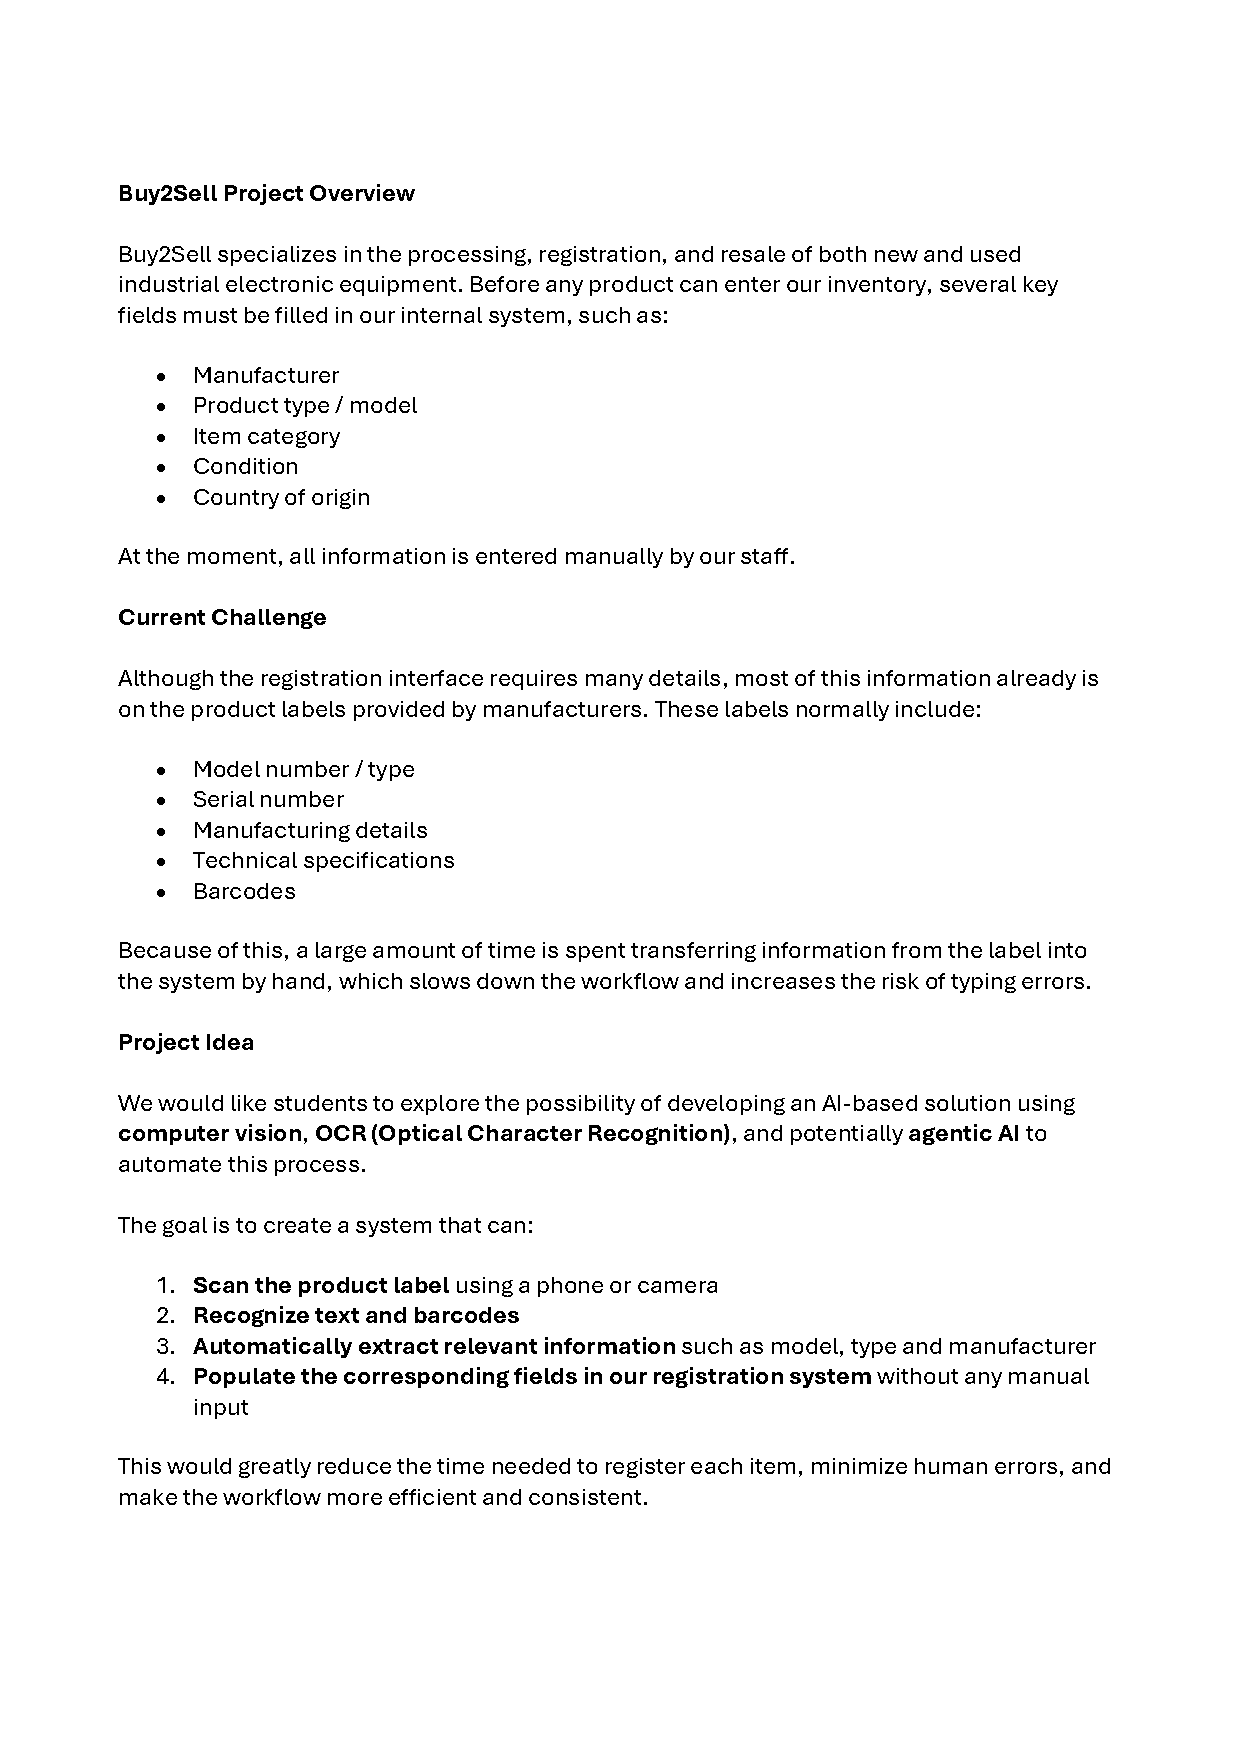
\includepdf[pages=-,pagecommand={}]{artifacts/buy2sell-project-overview.pdf}
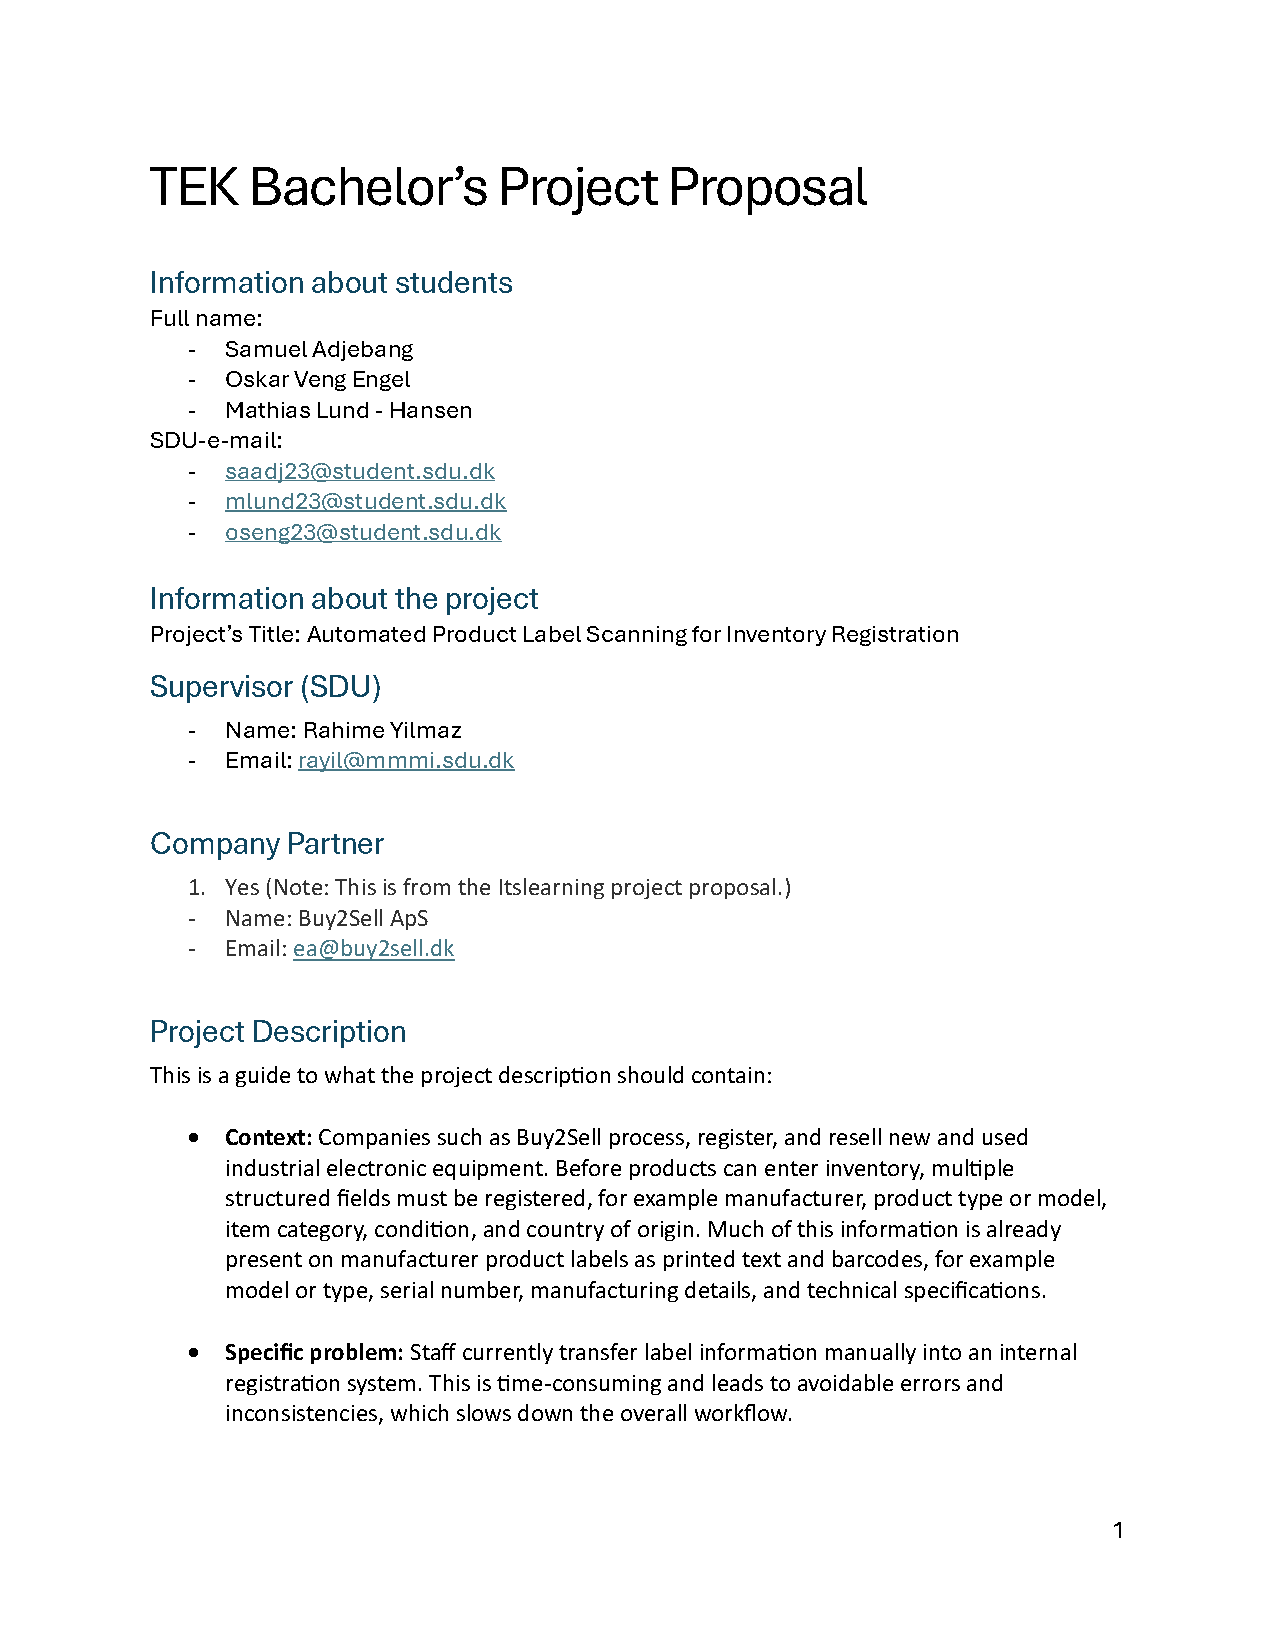
\includepdf[pages=-,pagecommand={}]{artifacts/english-se-bsc-rev2.pdf}
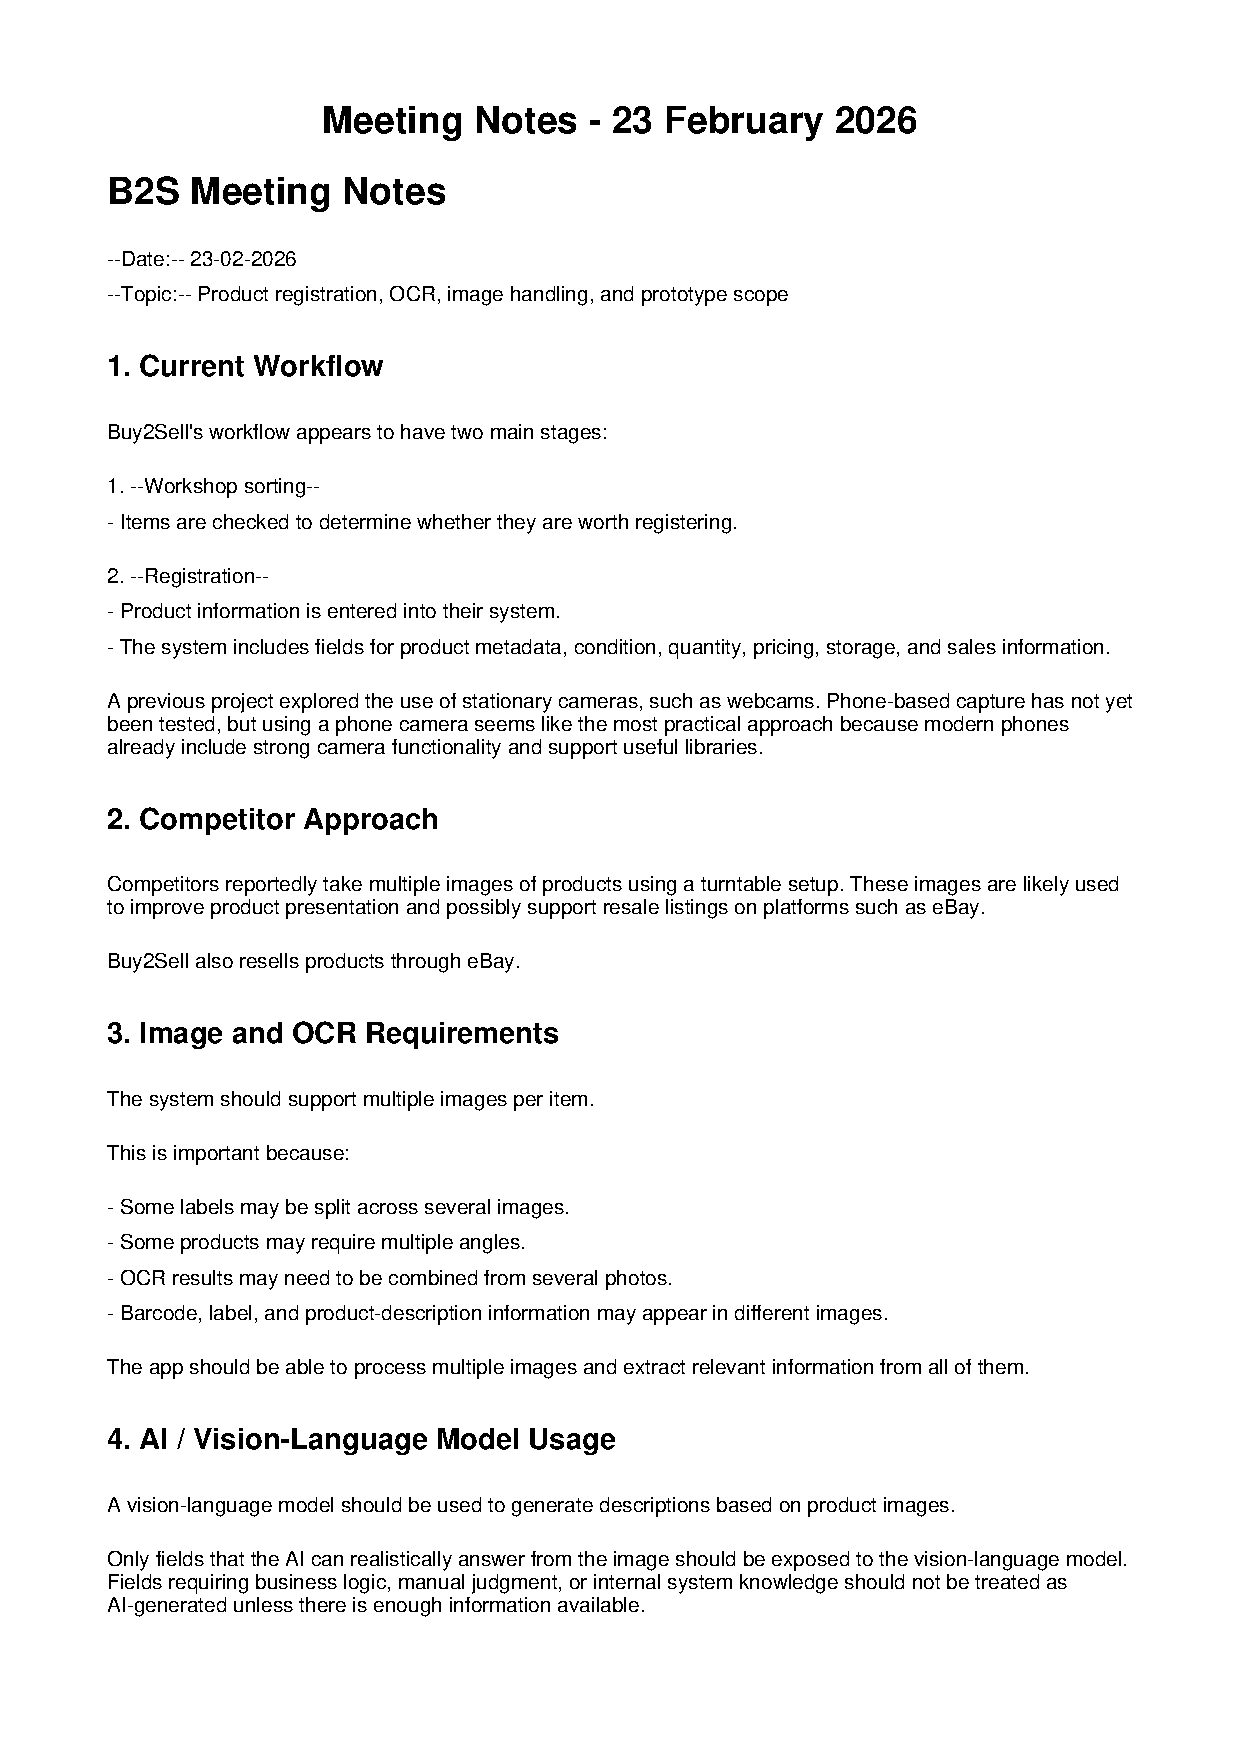
\includepdf[pages=-,pagecommand={}]{artifacts/meeting-notes-2026-02-23.pdf}
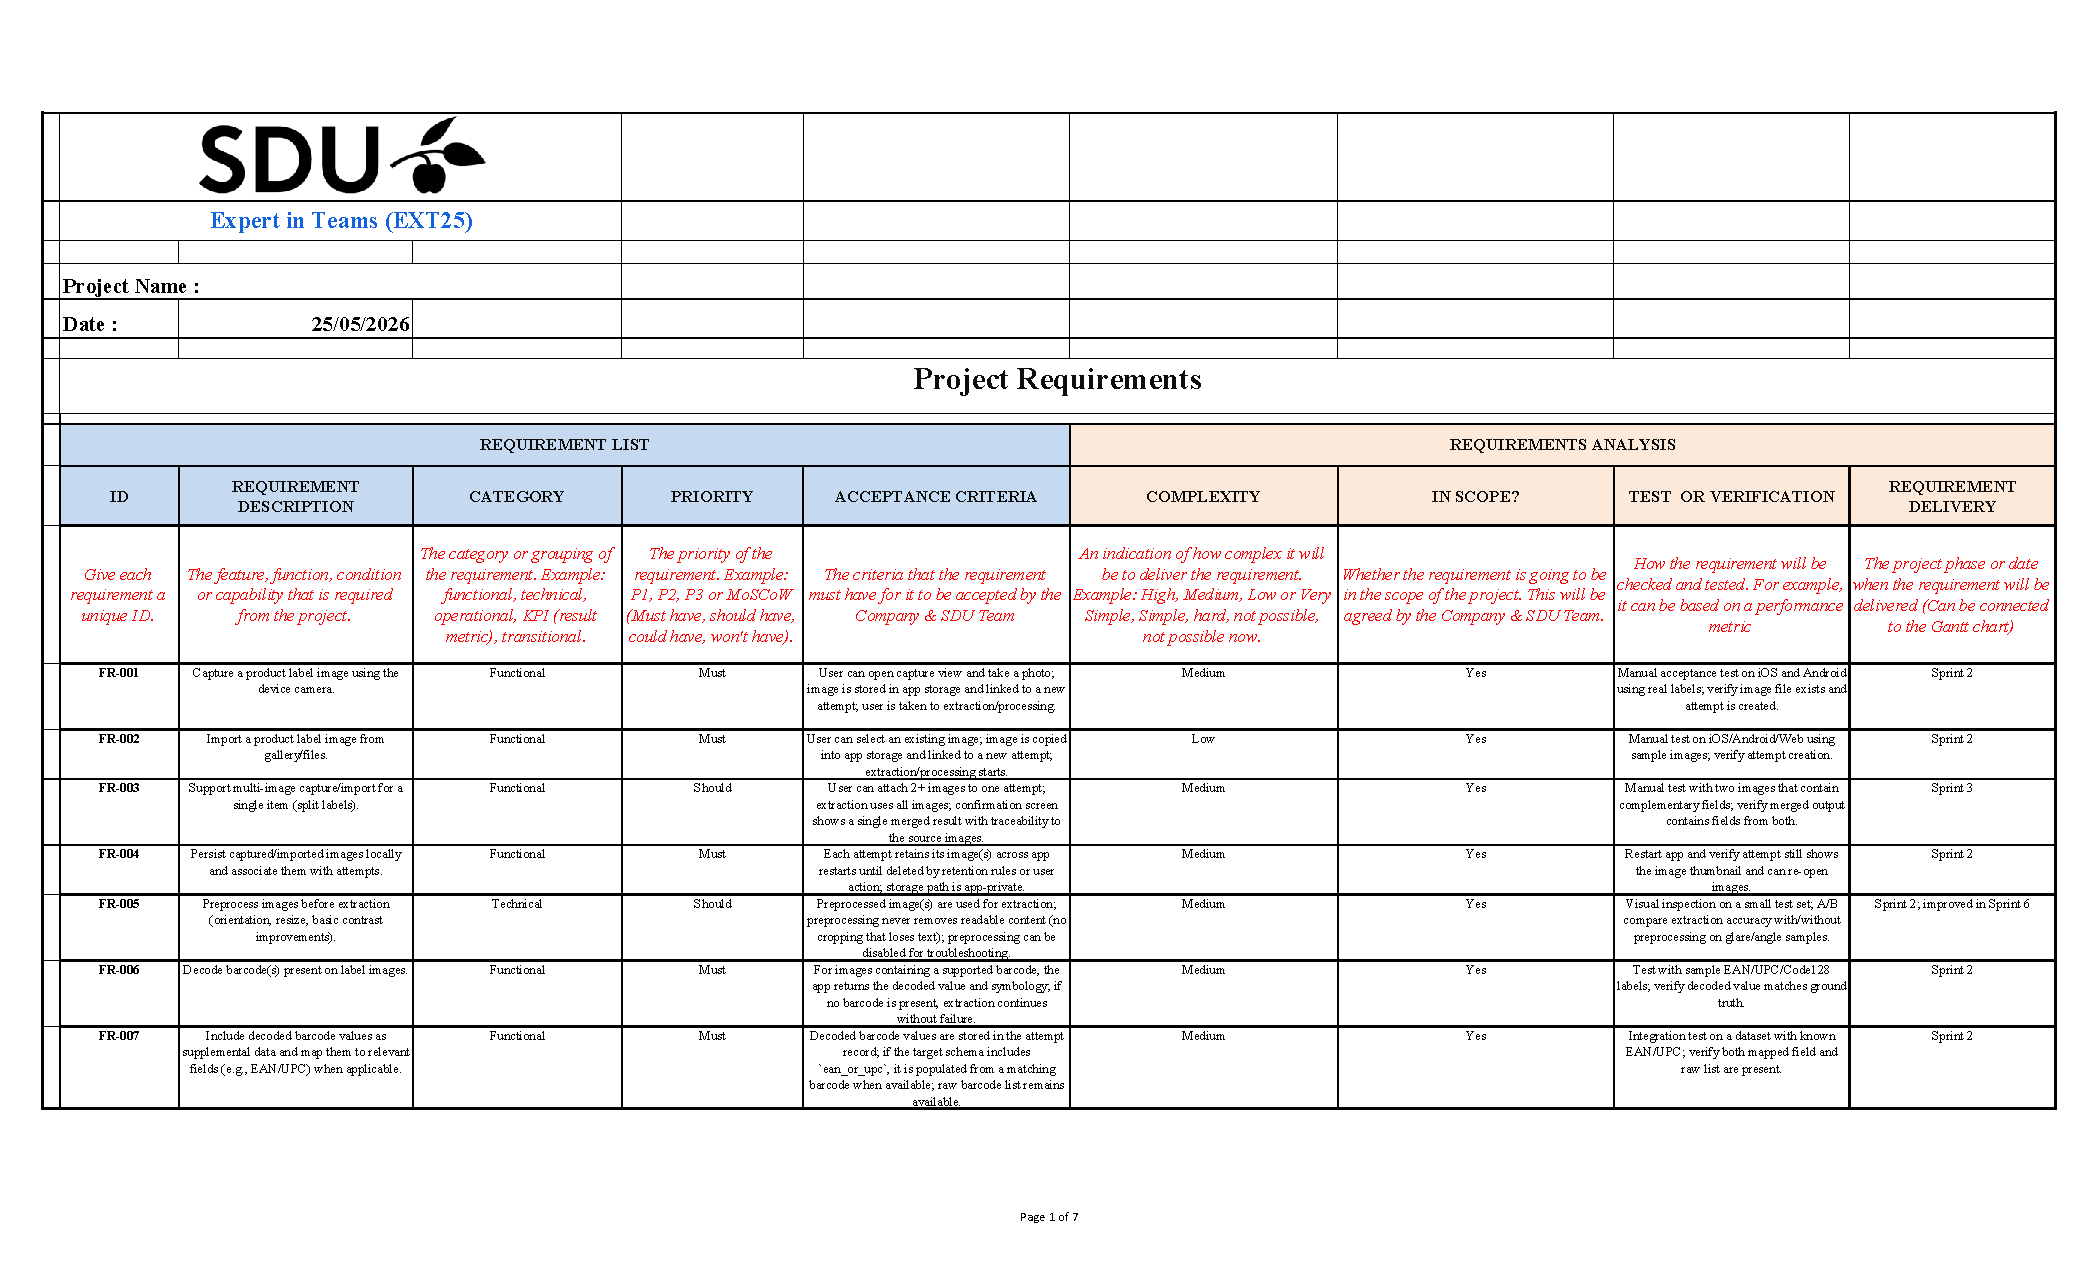
\includepdf[pages=-,pagecommand={}]{artifacts/project-requirements.pdf}
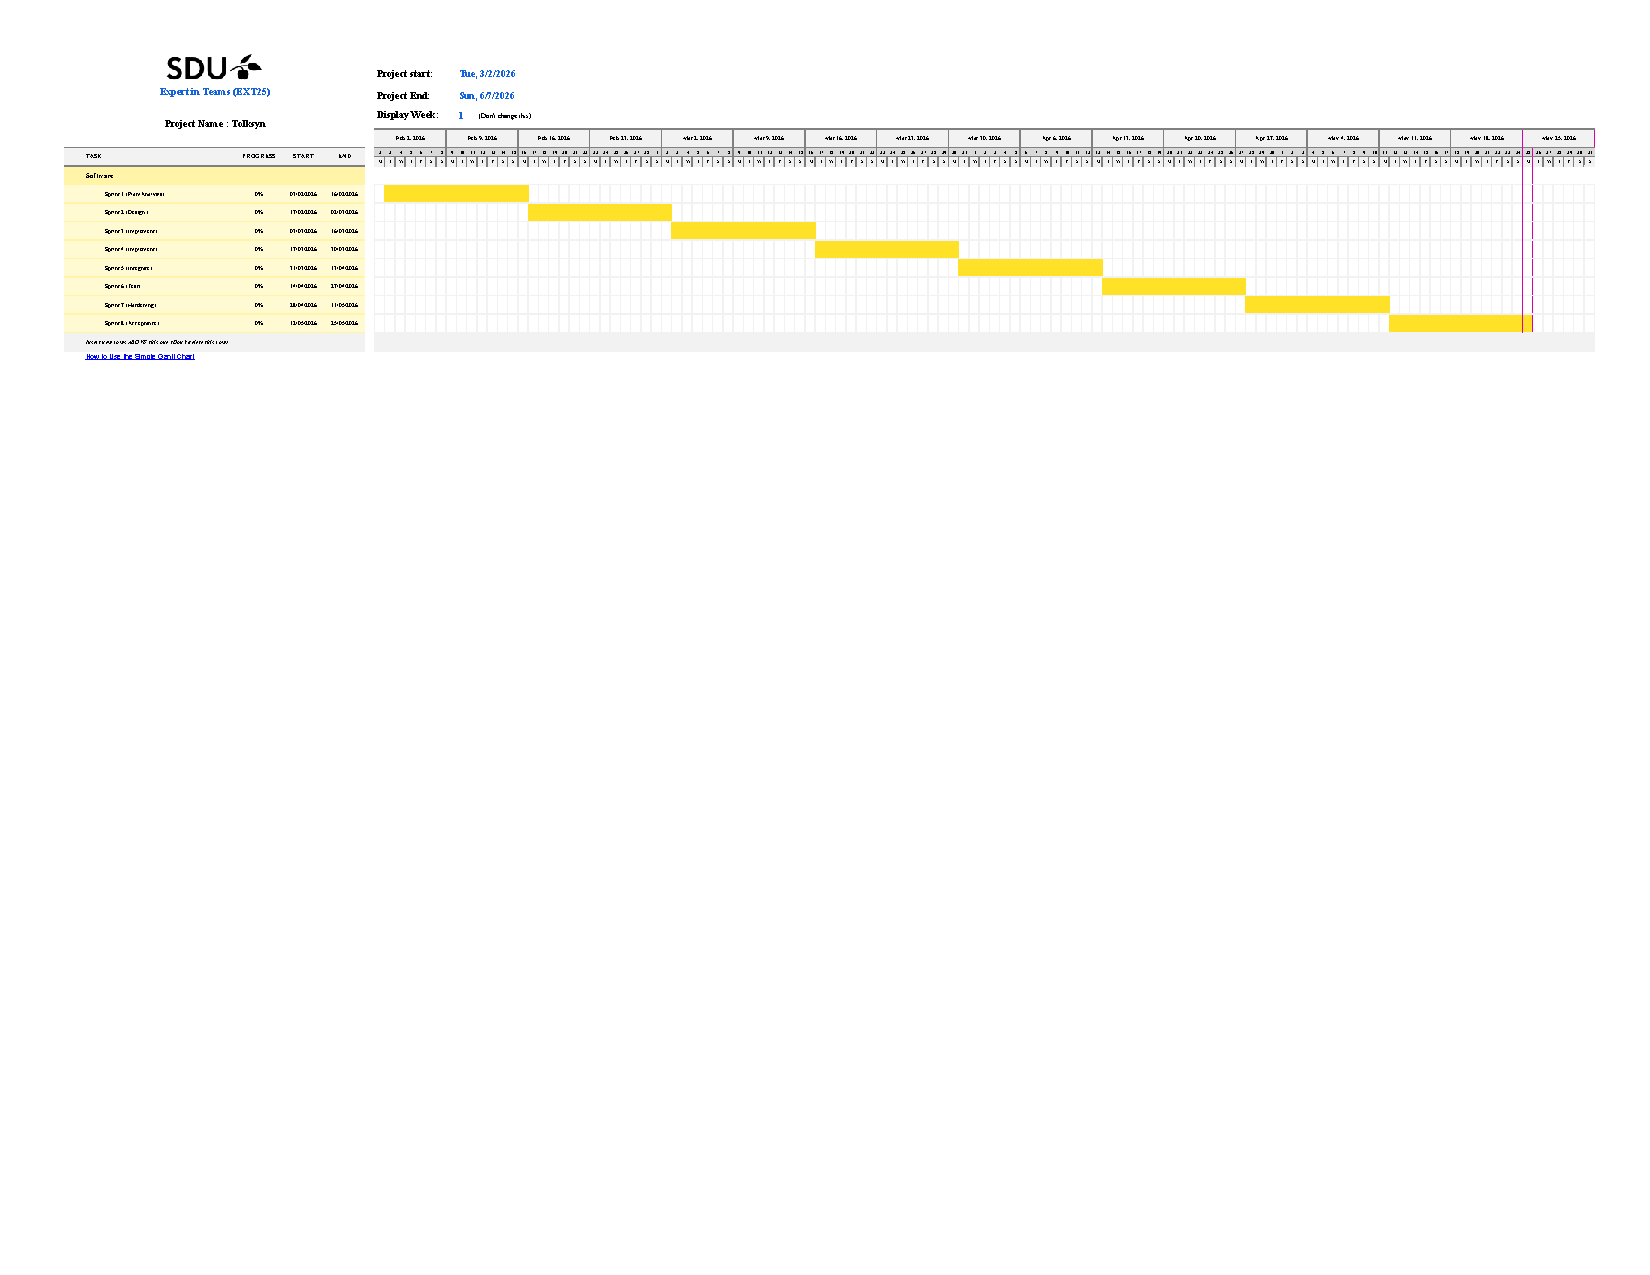
\includepdf[pages=-,pagecommand={}]{artifacts/gantt-chart.pdf}
% removed expo-app-folder-structure-best-practices.pdf
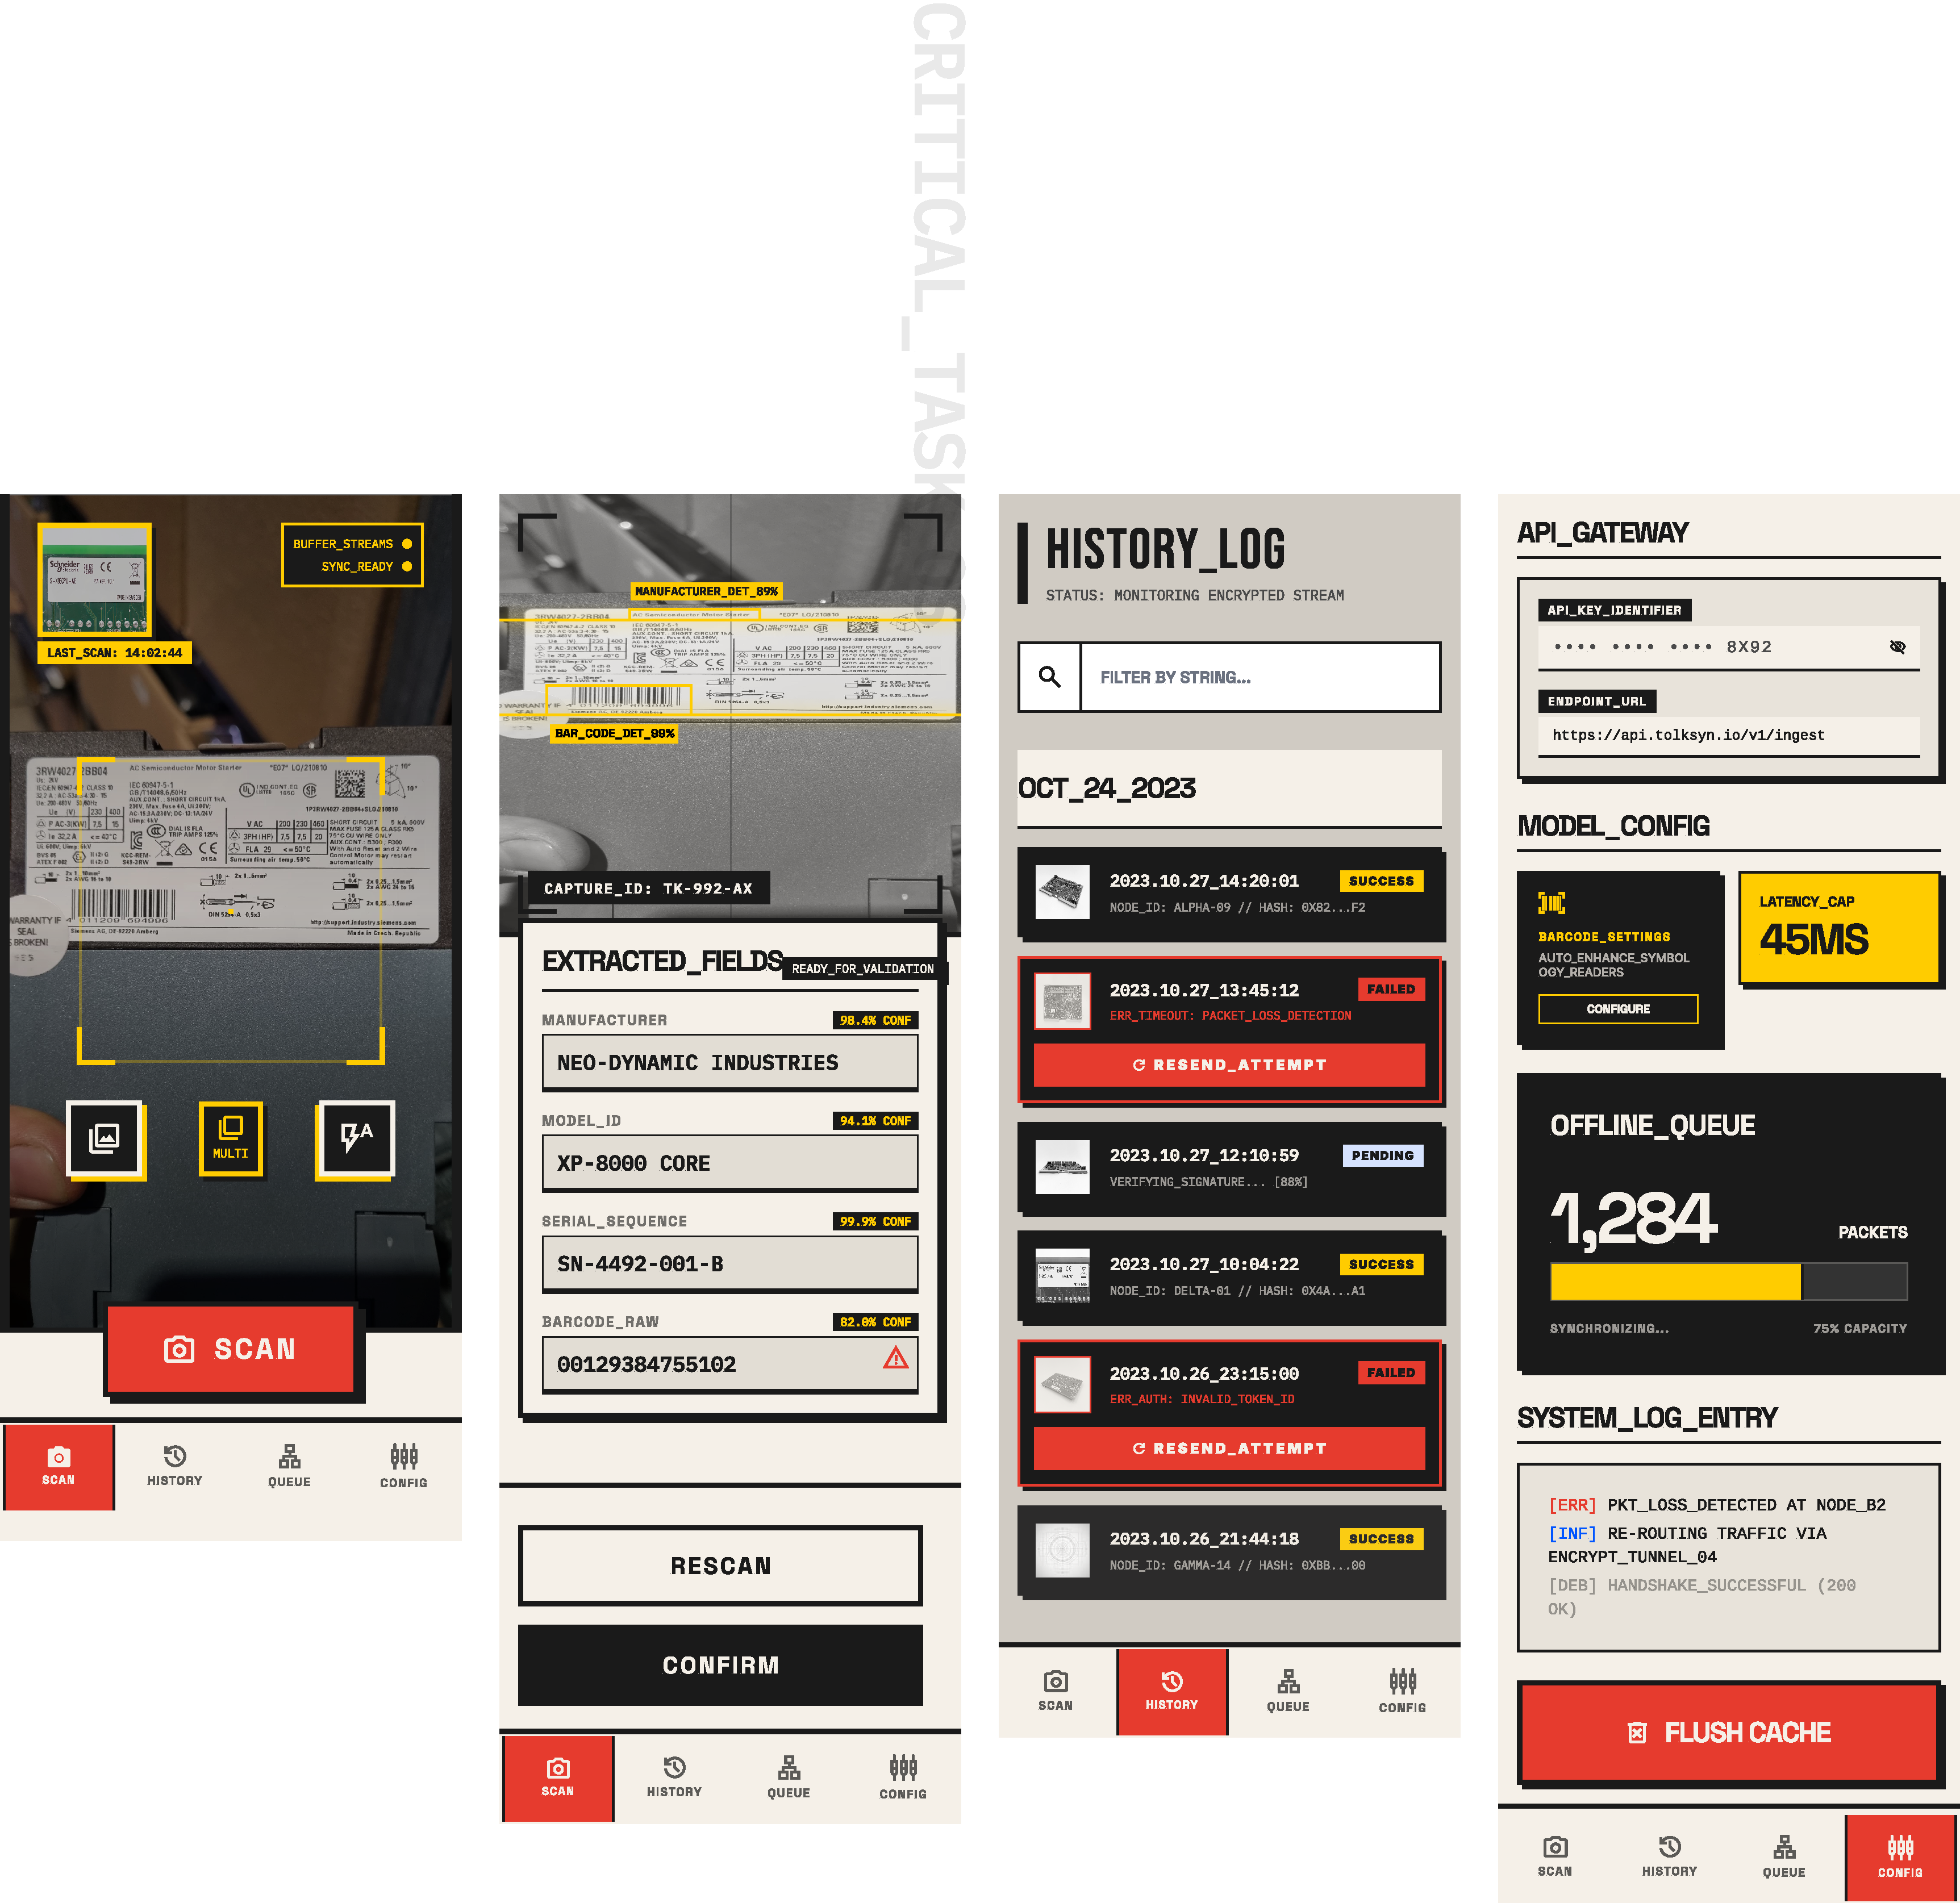
\includepdf[pages=-,pagecommand={}]{artifacts/figma-design.pdf}
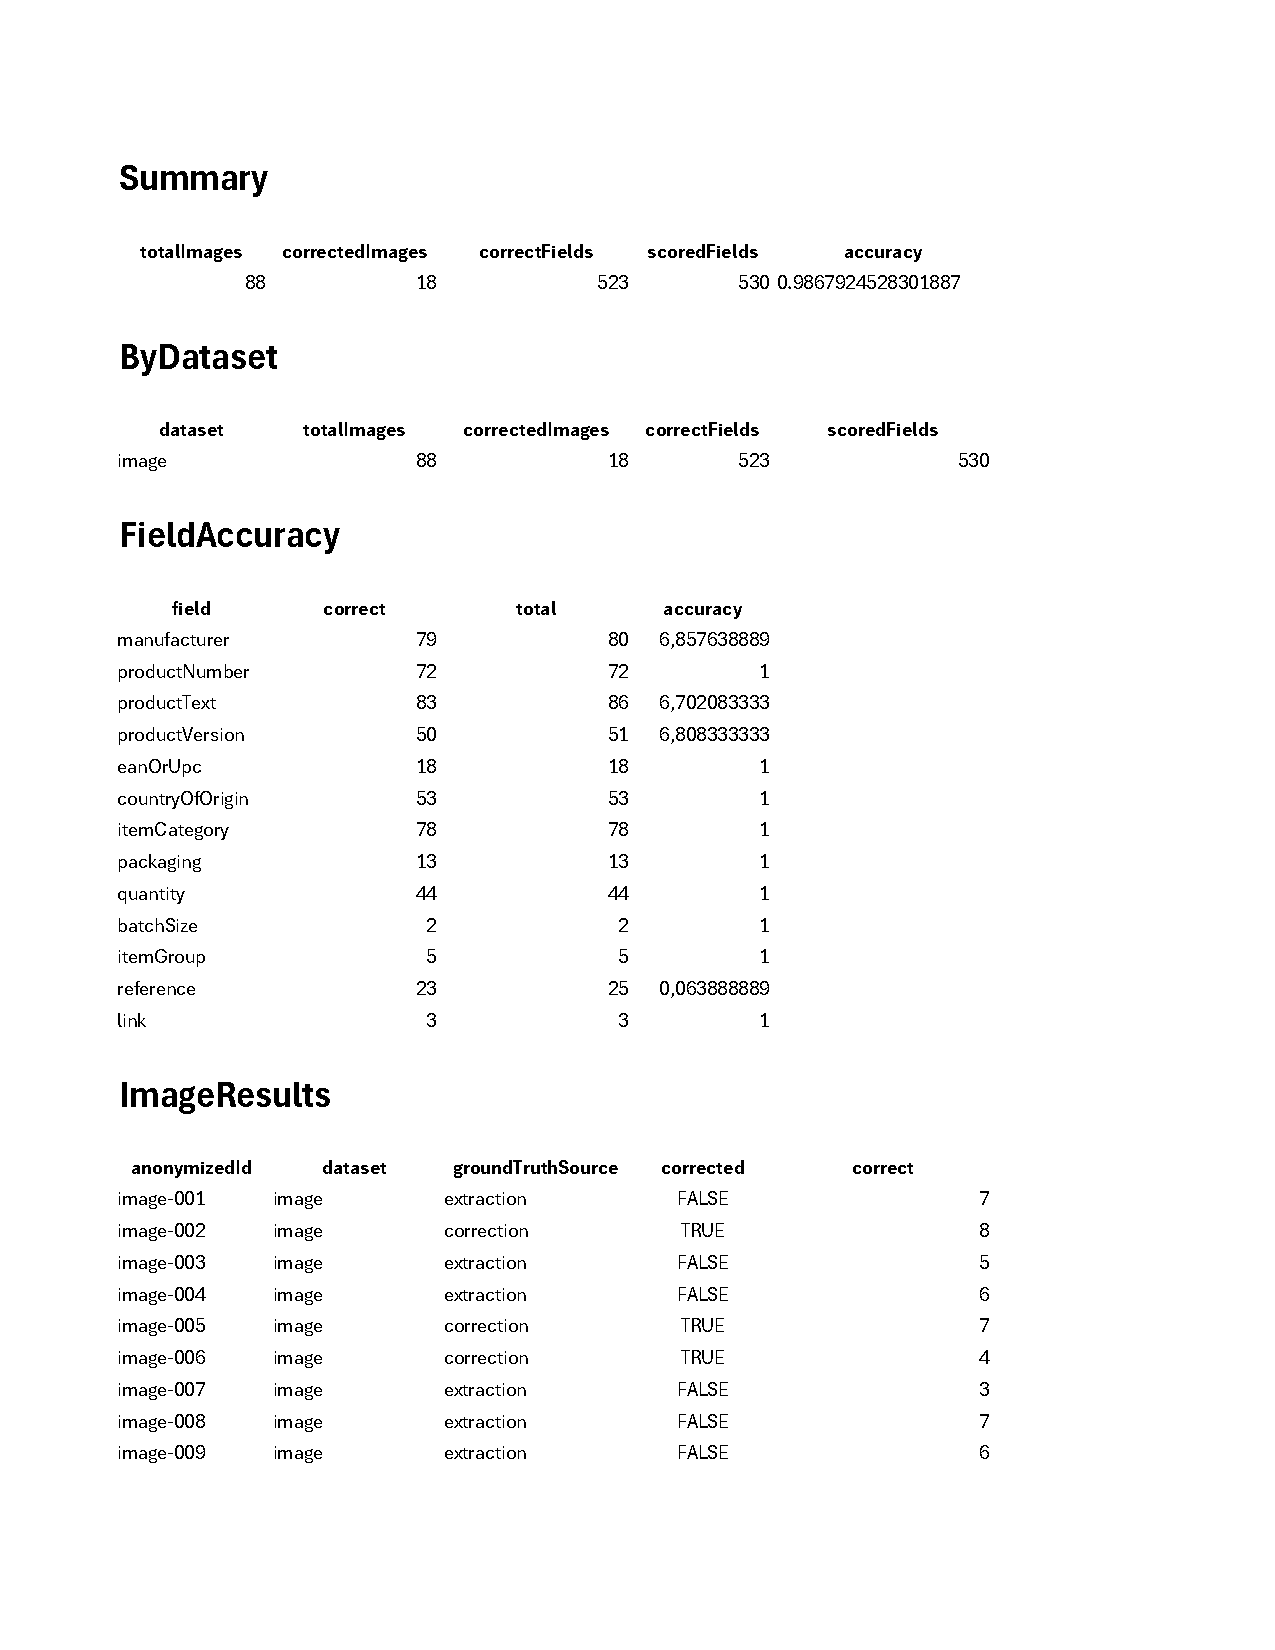
\includepdf[pages=-,pagecommand={}]{artifacts/kpi-anonymized.pdf}
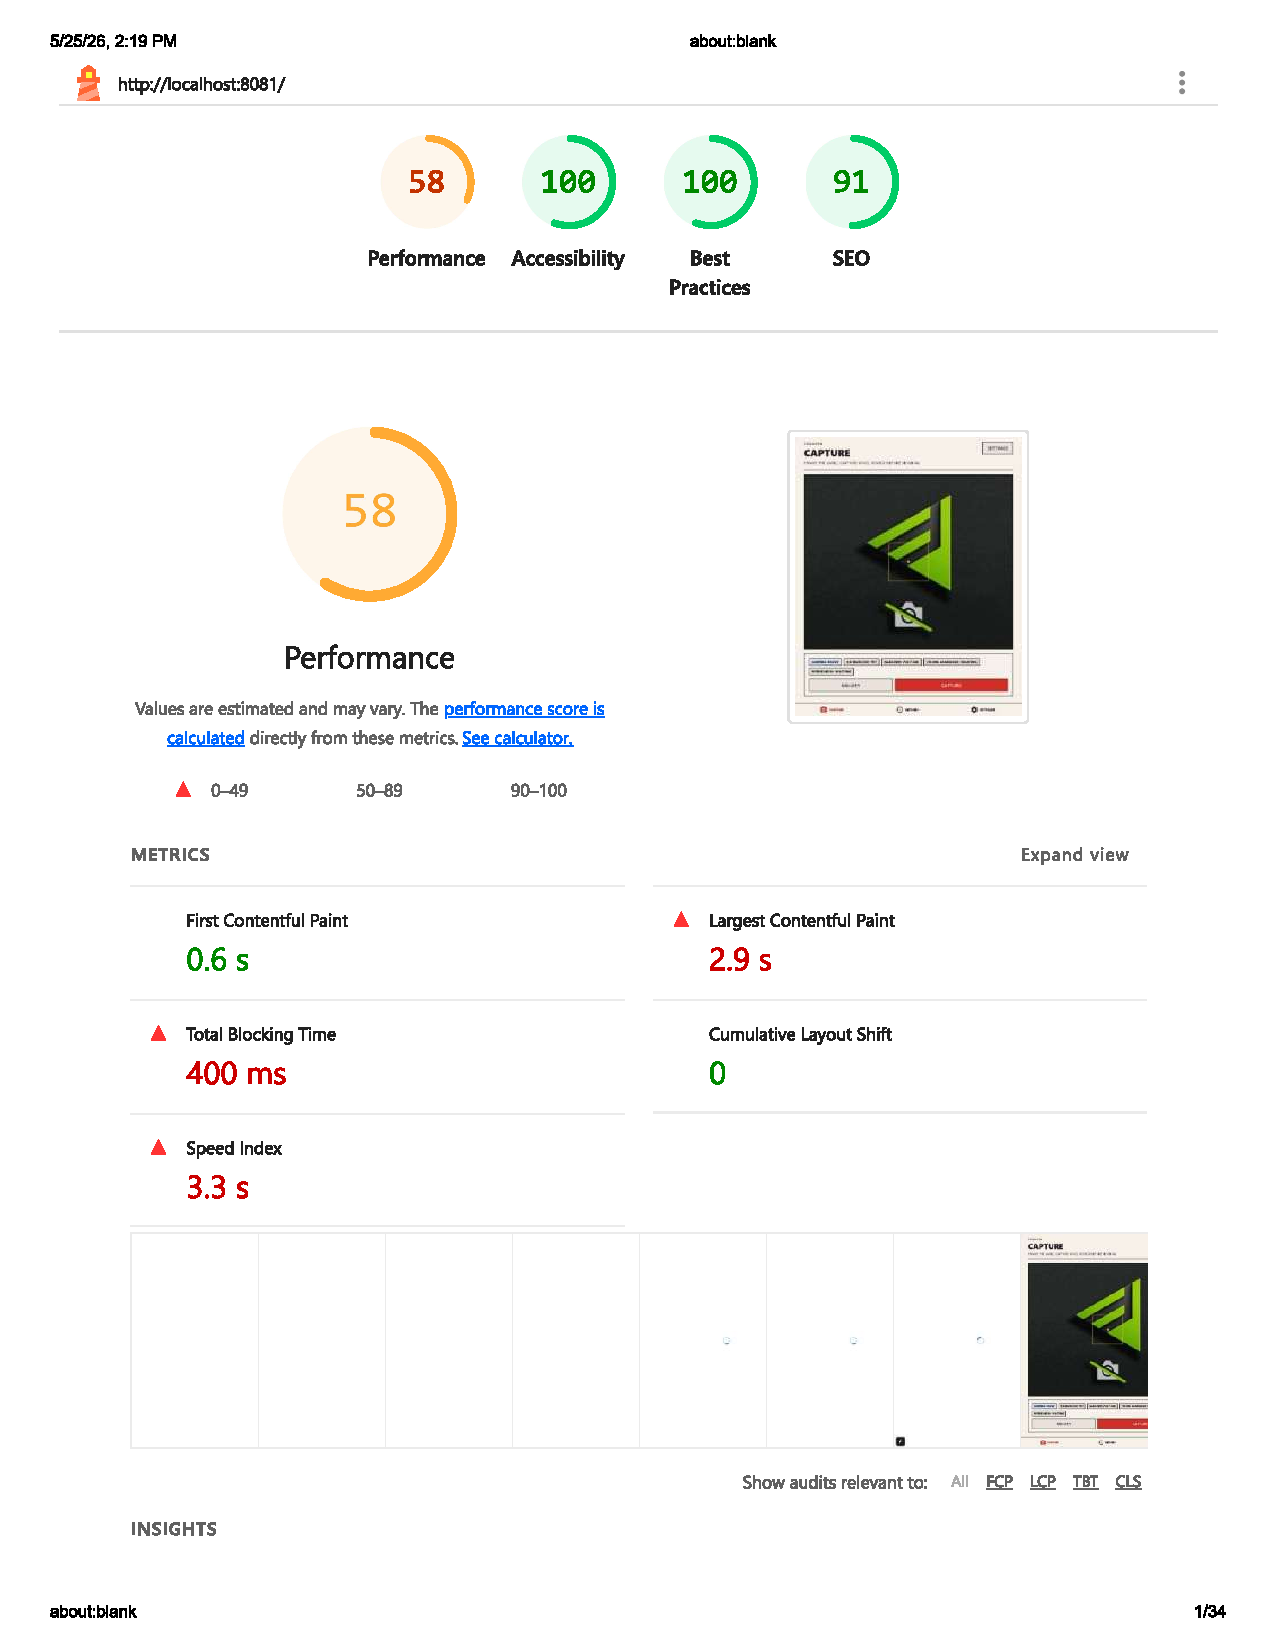
\includepdf[pages=1,pagecommand={}]{artifacts/lighthouse-capture.pdf}
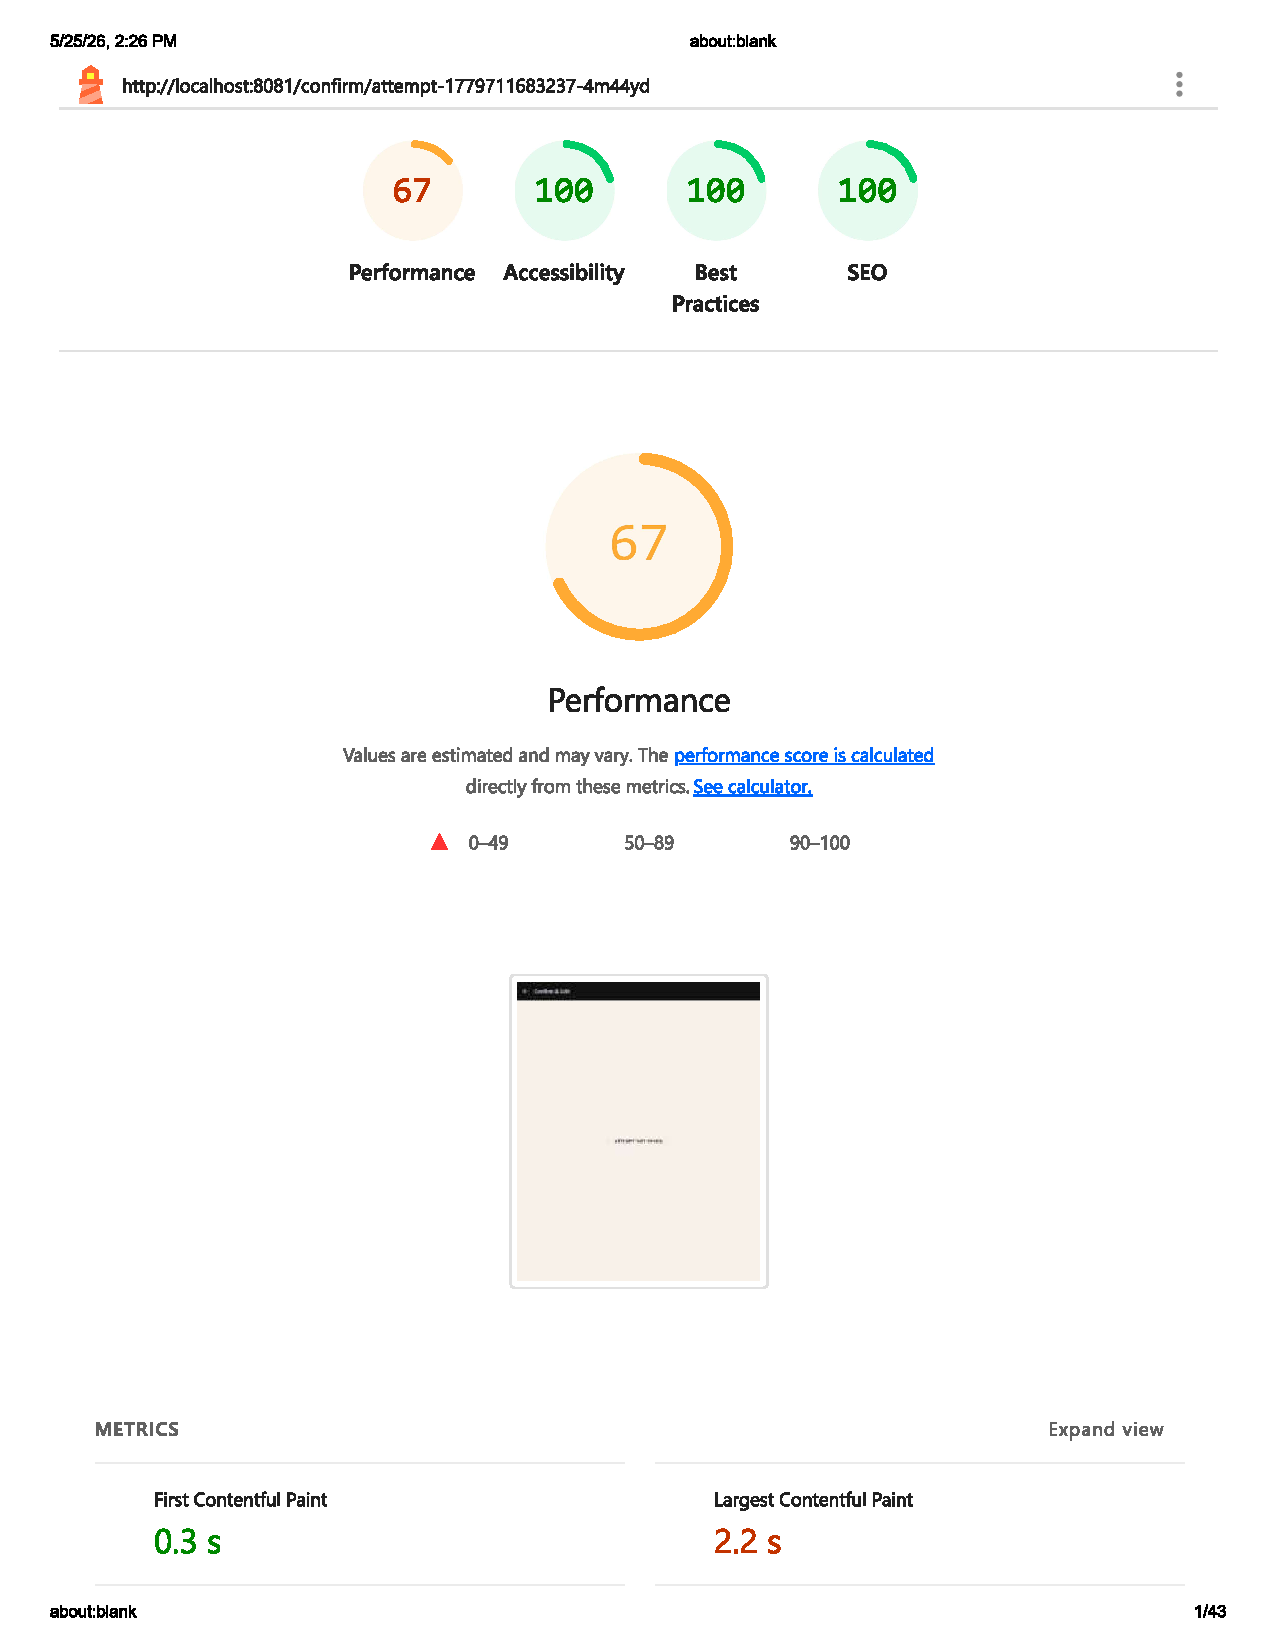
\includepdf[pages=1,pagecommand={}]{artifacts/lighthouse-confirm.pdf}
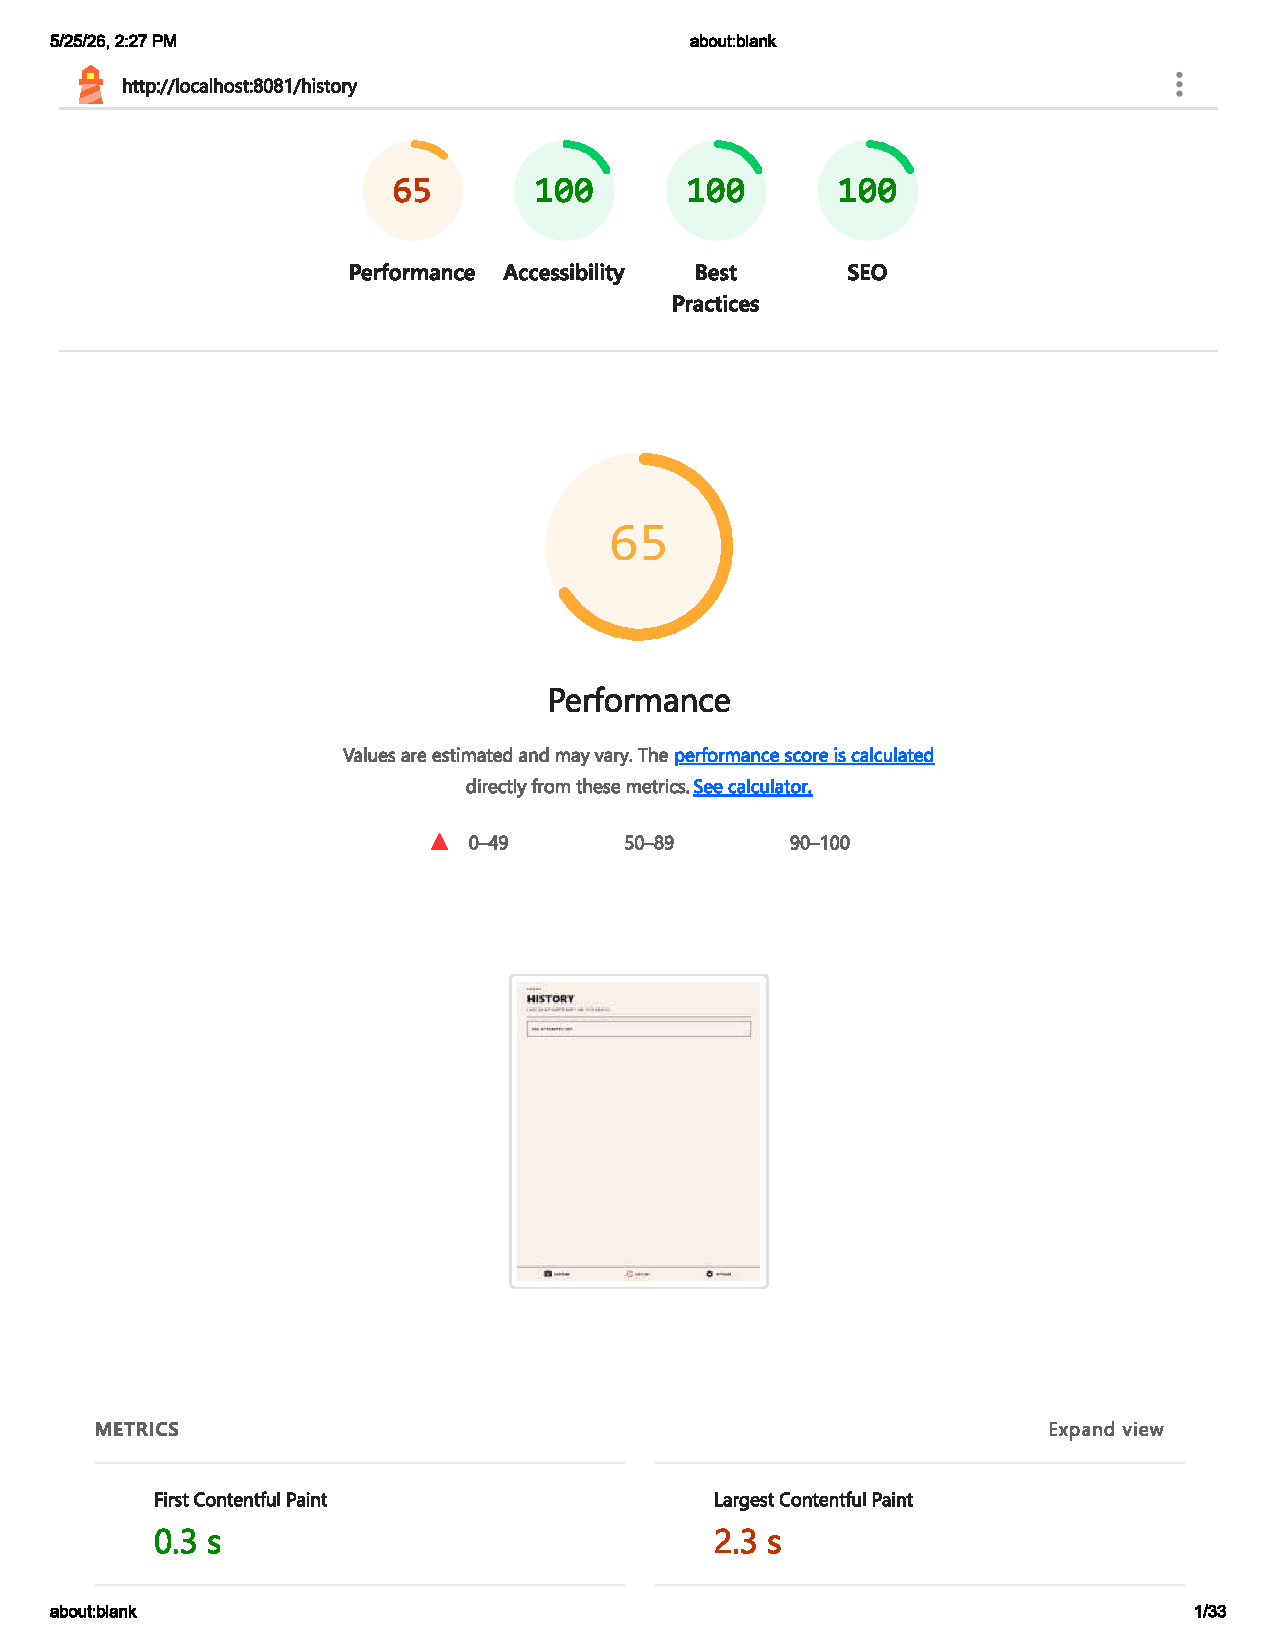
\includepdf[pages=1,pagecommand={}]{artifacts/lighthouse-history.pdf}
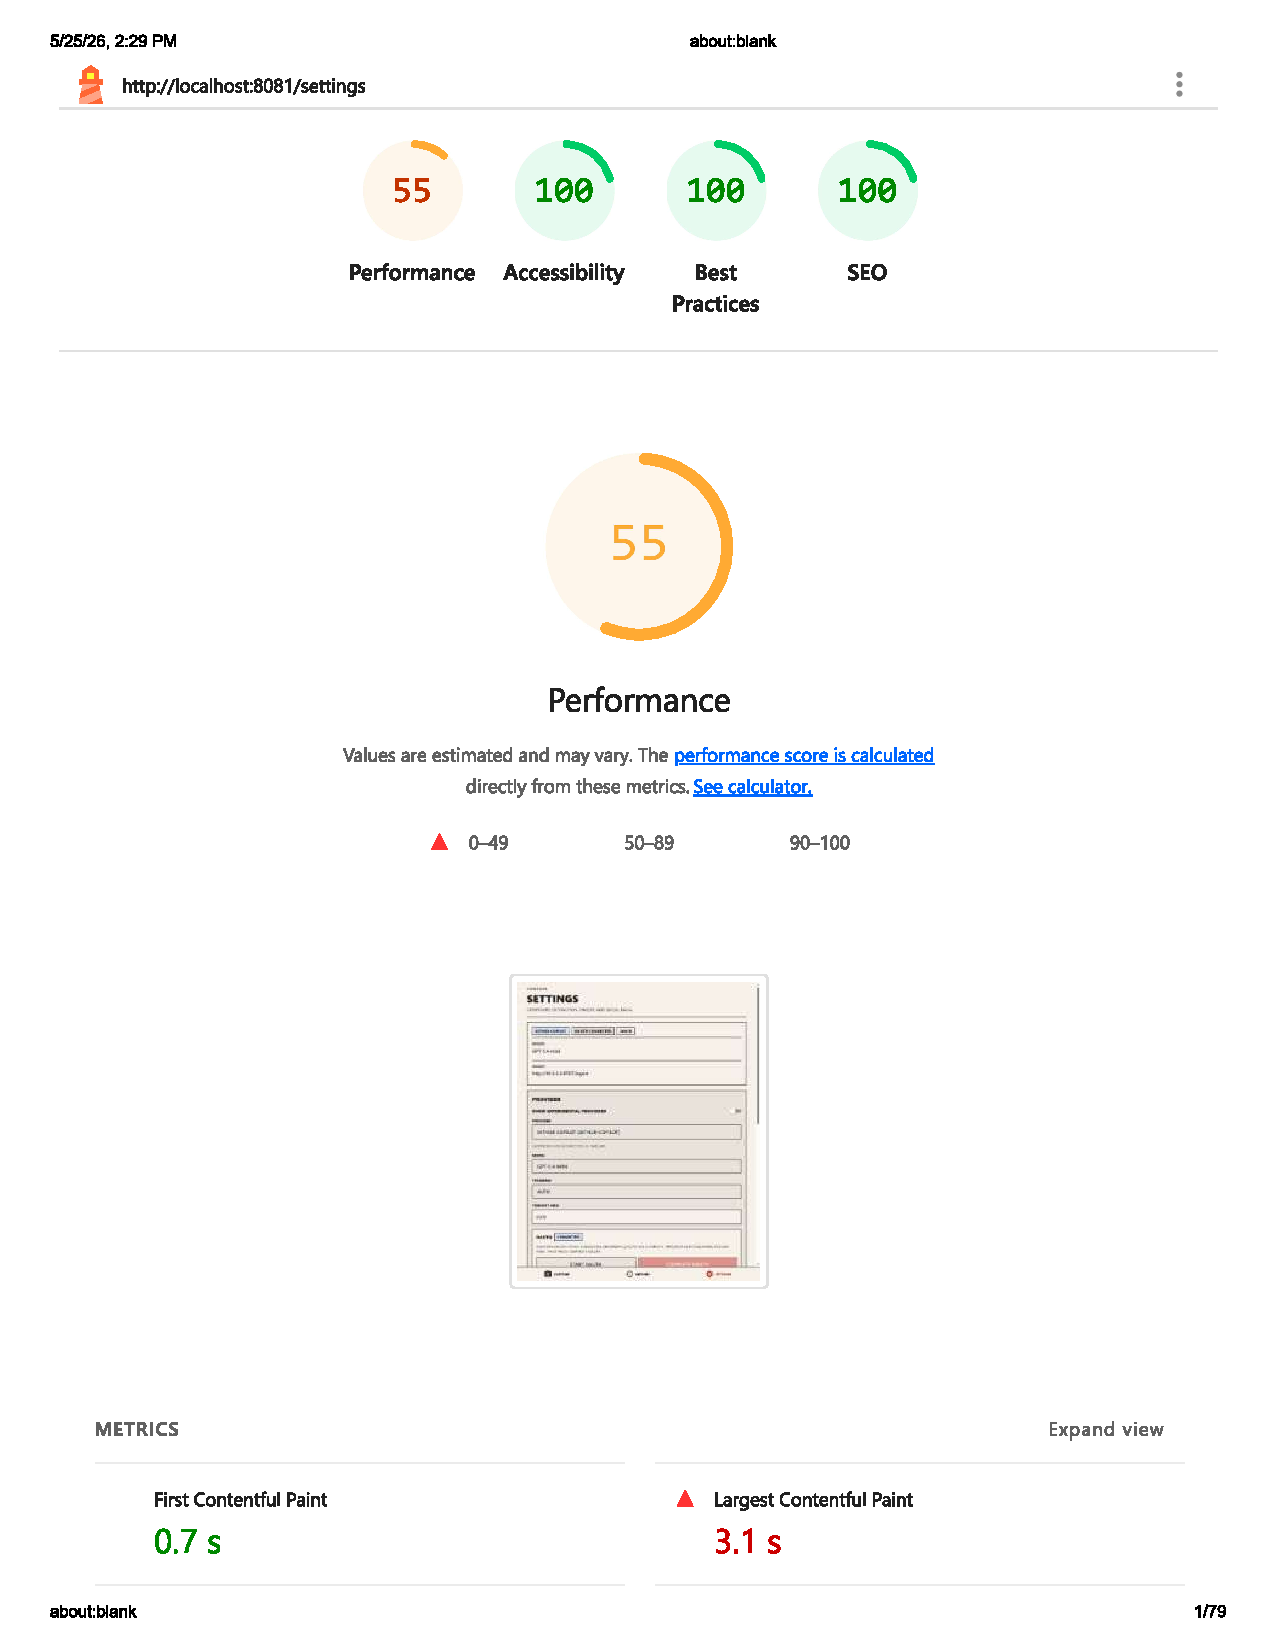
\includepdf[pages=1,pagecommand={}]{artifacts/lighthouse-settings.pdf}


\bibliographystyle{plain}
\bibliography{mybibliography}

\end{document}
